
\documentclass[draft]{agujournal2019}
\usepackage{url} 
\usepackage{lineno}
\usepackage[inline]{trackchanges} 
\usepackage{soul}
\usepackage{graphicx}
\usepackage{array}
\usepackage{amssymb} % various useful mathematical symbols
\usepackage{gensymb} % for `degree' sign
\usepackage{amsthm}  % extended theorem environments
\usepackage{lineno}   % for line numbers
\usepackage{amsmath} % for math operations
\usepackage{mathtools} % for math operations
\usepackage{tabularx} % for adjustable table width
\usepackage{amsmath}
\usepackage{xcolor}
\usepackage{epsfig}
\usepackage{multirow} 
\usepackage{colortbl}
\usepackage{adjustbox}
\usepackage{blindtext}
\usepackage{ragged2e}

\linenumbers
%%%%%%%
% As of 2018 we recommend use of the TrackChanges package to mark revisions.
% The trackchanges package adds five new LaTeX commands:
%
%  \note[editor]{The note}
%  \annote[editor]{Text to annotate}{The note}
%  \add[editor]{Text to add}
%  \remove[editor]{Text to remove}
%  \change[editor]{Text to remove}{Text to add}
%
% complete documentation is here: http://trackchanges.sourceforge.net/
%%%%%%%

%\draftfalse


\journalname{JGR: Solid Earth}


\begin{document}


\title{Modelling precursory laboratory seismicity using a roughness-based rate- and state-dependent friction model}


\authors{P.A. Selvadurai \affil{1}, P. Galvez \affil{2}, P.M. Mai \affil{2}, S.D. Glaser \affil{3}, D.B. Peter \affil{2} and S. Wiemer \affil{1}}



\affiliation{1}{Swiss Seismological Service, ETH Zurich, Zurich, Switzerland}
\affiliation{2}{King Abdullah University of Science and Technology, Thuwal, Saudi Arabia}
\affiliation{3}{Civil and Environmental Engineering, University of California, Berkeley, California, USA}

\correspondingauthor{Paul A. Selvadurai}{paul.selvadurai@sed.ethz.ch}




\begin{keypoints}
\item Rate and state friction (RSF) models were developed from roughness measurements of a friction experiment that displayed properties of wear
\item Simulations showed that smooth sections nucleated events that ruptured and were arrested by local roughened sections representing barriers
\item Source properties of the RSF ruptures were compared to independently measured kinematic estimates from a concerted study for the first time
\end{keypoints}


\begin{abstract}
We investigate experimental results from a direct shear friction apparatus, where a fault was formed by pressing mature, worn surfaces of two polymethyl methacrylate (PMMA) samples on top of each other in a dry environment. The fault was sheared until macroscopic stick-slip frictional failure occurred. Before the macro-failure small precursory seismicity nucleated from regions that also experienced aseismic slow slip. These precursory events did not cascade-up into gross fault rupture and arrested locally. Reasons as to why ruptures arrested are investigated using a 1-D rate and state friction (RSF) model. Surface profilometry of the fault surface taken \textit{a posteriori} revealed wear in the form of a bimodal Gaussian distribution of surface height. In our model, this unique distribution of surface roughness is determined to be a proxy for the heterogeneous spatial description of the critical slip distance $D_{c}$. We assume that smooth (polished) sections of fault exhibited lower $D_{c}$ than rougher sections of the bimodal Gaussian roughness profile.  We used a quasi-dynamic RSF model that determined localized seismicity initiated at the smooth sections. Source properties: average slip $\delta$, seismic moment $M_{0}$, stress drop $\Delta \tau$ and fracture energy $G^{'}$, were determined for each event. We compare the numerically modeled source properties to experimental source characteristics inferred from seismological estimates using an array of acoustic emission sensors from a concerted study. We discuss similarities, discrepancies and assumptions between these two independent models (kinematic and dynamic) used to study earthquakes for the first time in the laboratory.
\end{abstract}

\section*{Plain Language Summary}
Recent seismic observations show that faults experience a range of slip patterns spanning many scales in both space and time. Understanding how slip accumulates on complex fault systems can lead to a better understanding of regions that are more prone and susceptible to large events.

We studied a scaled version of a frictional fault laboratory. This fault also showed complex slip behavior. We notice that scaled versions of earthquakes occurred in larger regions that were also slipping more slowly. This behavior has also been observed in nature but we are not certain as to why exactly. We linked this behavior to a mathematical model that describes friction on faults. To add complexity, we used the experimental roughness measured along the interface, which might explain the complicated slip patterns. Using the roughness, we found that the model produced earthquakes patterns and general behaviors that matched many experimental measurements taken independently. We found that complexity formed by fault roughness can produce a wide range of slip behaviors that are also observed in natural systems at many scales. Understanding how roughness evolves over a fault's lifetime will be important for moving forward earthquake science.  


%\begin{keyword}
%Laboratory seismology, Slip spectrum, Earthquake nucleation and arrest, Rate and state friction, Asperities, Source properties
%\end{keyword}


\section{Introduction}
\label{int}
Growing amounts of seismologic observations capture an ever larger diversity in slip behavior along natural faults. Over recent years seismologists have reported the occurrence of slow earthquakes \cite{Ide2007, Beroza2011} and it is now commonly accepted that slip happens over different length and time scales \cite{Peng2010}. Slow earthquakes themselves have been observed to have a wide range of slip behaviors and radiation patterns. Due to the close spatial proximity of slow earthquakes to massive megathrust earthquakes, connecting the physical impact of these slow processes imposes on regions of the fault that is historically susceptible to fast sliding on large scales.  Having insight in these connections is critical to developing a better understanding of the entire earthquake cycle \cite{Obara2011, Obara2016}. 
 
It is believed that slow and fast earthquakes share a common slip mechanism \cite{Obara2016}.  Slow slip is also believed to occur in the nucleation phase associated with the onset of frictional instability (also known as the premonitory or preslip phase).  The preslip phase has sometimes been identified in the onset of the mainshock seismogram \cite{Iio1995, Ellsworth1995}. Detection of a nucleation phase at regional scales (kms) using the onset of seismograms is difficult since it resides at the lower thresholds of seismologic capabilities \cite{Tullis1996}. Recent improvements in geodetic measurements (GPS, InSAR) have been able to  lower the detectable threshold and identify this phase over long time scales (months to years) and length scales (kms) \cite<e.g.>[]{Brodsky2014, Ruiz2014, Socquet2017}.  The nucleation phase and associated premonitory slip is well observed in laboratory experiments on frictional faults \cite{Dieterich1978, Ohnaka1999, Nielsen2010, Latour2013, McLaskey2013, Selvadurai2015} but remains debated as to whether it exists universally in highly complex structures such as fault cores \cite<e.g.>[]{Chester1993, Mitchell2009}.  
 
In this study, we focus on what controls the occurrence of foreshocks (or precursory seismicity) in the nucleation phase of laboratory ruptures. Laboratory studies suggest that asperities (i.e. frictional heterogeneity) exist on the fault \cite{Selvadurai2015, Selvadurai2017}. One mechanism for foreshocks is that as a preslip region grows larger it accelerates, the increased stressing rate might contribute to the dynamic failure of these asperities \cite{McLaskey2013}.  Another hypothesis is that asperities have higher levels of normal stress, thus locally decreasing its critical nucleation distance and if the asperity is geometrically large enough it could potentially lead to dynamic failure in the presence of preslip \cite{Veedu2016, Selvadurai2017, Schaal2019}.  Studies of the initial onset of seismicity appear to indicate that asperities, which exist at smaller spatial scales, even on natural faults, might provide the initial trigger leading to fault failure at larger spatial scale \cite{Iio1995, Ellsworth1995, Beroza1996, Okuda2018}.  This type of hierarchical breakdown may be indicating the possible existence of a hierarchical plate interface structure.  Foreshocks might be local failures of these asperities that do not fully `cascade-up’.  

Reasons as to why foreshocks arrest and do not always culminate in large earthquakes are not well understood so far. We believe that ruptures begin to expand in a crack-like manner, then accelerate outwards to a critical velocity, whereby they may transition to a pulse-like dynamic rupture \cite{Heaton1990, Meier2016}.  The mechanism behind whether a rupture transitions from a crack-like to pulse-like rupture is not well understood and may depend on numerous factors such as heterogeneous presence of frictional barriers or prestress \cite{Rubinstein2004, Maegawa2010, Tromborg2011, Kammer2012, Otsuki2013, Kammer2015, Selvadurai2017a, Ke2018}. In this study, we assume that the presence of both fast and slow rupture occur in the same region arises from and around asperities formed by topographic mismatch of the two rough surfaces in our laboratory setting.

This study is separated into two parts: (\textit{i}) Surface roughness is measured over a range of length scales using metric from interdisciplinary fields of contact mechanics, tribology and geophysics. (\textit{ii}) We use the experimental surface roughness measurements, to develop a dynamic friction model that obeys the rate and state friction (RSF). Part (\textit{ii}) will help us reconcile the seismically observed laboratory foreshocks \cite{Selvadurai2019}. The RSF model investigates the concept that heterogeneity is a prerequisite for having synchronous slow and fast rupture on similar sections of a fault. In our model this was imposed by assuming variable $D_{c}$ along the modeled region. Spatial fluctuations in fault roughness -- smoother and more rough sections -- assumed properties based on arguments that follow past laboratory observations \cite{Marone1994, Marone1998}. Smooth sections were prescribed as lower $D_{c}$, whereas rough section were given higher levels of $D_{c}$. This assumption is based on numerical modelling that explains $D_{c}$ in terms of the micromechanics governing friction on dry, gouge-free interfaces \cite{Yoshioka1996}. 

The model developed here was used to simulate a range of experimental conditions that concomitantly produced localized seismicity and aseismic slip on the fault. Seismic source properties were extracted from a quasi-dynamic RSF numerical model and compared to estimates made from the spectral analysis of the seismic waves in a supporting study \cite{Selvadurai2019}. With our frictional model we investigate some open questions: (\textit{i}) How does the level of strength heterogeneity or the evolving stress field affect rupture initiation, propagation and arrest? (\textit{ii}) How does this affect estimates on dynamic source properties? And (\textit{iii}) How does kinematic estimates compare to dynamic rupture model with an implicit prescription of heterogeneity through roughness?

%%%%%%%%%%%%%%%%%%%%%%%%%%%%%%%%%%%%%%%%%%%%%%%%%%%%%%%%%%%%%%%%%%%%%%%%%%%%%%%%%%%%%%%%%%%%%%%%%%%%%%%%%%%%%%%%%%%%%%%%%%%%%
\section{Experimental Methods and Results}
\subsection{Material Properties}
\label{MaterialProperties}
Physical properties of PMMA at room temperature are:  Shear modulus $G$ = 2.39 x 10$^9$ Pa, Poisson's ratio $\nu$ = 0.32 and $\rho$ = 1180 kg m$^{-3}$.  Using a Rockwell B Hardness test the indentation yield strength was found to be $Y$ = 586 MPa and the independently performed differential scanning calorimetry (DSC) determined the glass transition to be $T_g$ = 114 $^o$C. The body and shear wave velocities of the material were $V_{P}$ = 2800 m s$^{-1}$ and $V_{S}$ = 1330  m s$^{-1}$, respectively, giving a ratio $V_{P}/V_{S} \approx$ of 2.1. 

%%%%%%%%%%%%%%%%%%%%%%%%%%%%%%%%%%%%%%%%%%%%%%%%%%%%%%%%%%%%%%%%%%%%%%%%%%%%%%%%%%%%%%%%%%%%%%%%%%%%%%%%%%%%%%%%%%%%%%%%%%%%%
\subsection{Surface Preparation}
\label{Surface preparation}
The interacting faces of the PMMA slider block and base plate were first sandblasted using 220-440 $\mu$m particles of aluminum oxide (Al$_2$O$_3$) for a controlled time, distance and pressure.  Sandblasting surfaces is routinely used to produce self-affine properties that are believed to occur during the generation of new faulting via the mechanism of tensile cracking \cite{Power1991, Schmittbuhl2006, Persson2014}.  Initial hand lapping of the surfaces with SiC abrasives \cite{Dieterich1994} will not result in worn surfaces resembling those formed by initially sandblasting then wearing the interface. According to \citeA{Persson2014}, surface lapping with sandpaper will roughen an initially flat surface without forming the high, sharp asperities.  The removal of material is easier at the top of the asperity than in the valley creating a rough surface with a low fractal dimension.  We believe that sandblasting the freshly machined samples of PMMA was necessary to obtain initial conditions, which upon being frictionally worn past each other exhibited the unique surface roughness and frictional behavior described in this study.

%%%%%%%%%%%%%%%%%%%%%%%%%%%%%%%%%%%%%%%%%%%%%%%%%%%%%%%%%%%%%%%%%%%%%%%%%%%%%%%%%%%%%%%%%%%%%%%%%%%%%%%%%%%%%%%%%%%%%%%%%%%%%
\subsection{Summarized General Findings}
\label{GeneralExp}

 A schematic diagram of the direct shear friction apparatus is shown in Figure \ref{fig1}(a). We refer to this scale as the macrosopic scale for the discussion. The reader is urged to consult \citeA{Selvadurai2015a} and \citeA{Selvadurai2015} for a more detailed description of the experimental facilities. Full computer aided drawings (CAD) of the all components direct shear apparatus and their technical drawings are given in \citeA{Selvadurai2015b}. Experiments consisted of loading a long slender PMMA slider (12.7 mm x 406 mm x 80 mm) onto a larger PMMA base plate (610 mm x 305 mm x 51 mm). During an experiment, the fault was maintained under constant normal load $F_{n}$.  The top slider was driven at a constant macroscopic loading rate $V_{LP}$ and an in-line shear load cell was used to measure the bulk frictional resistance along the fault.  
 
 Figure \ref{fig1}(b) shows a typical experiment where the macroscopic loading rate was $V_{LP}$  = 0.010 mm s$^{-1}$ and the normal force was fixed at $F_{n}$ = 4400 N.   We note that the shear force increased until a large dynamic release, or stick-slip event, occurred.  This type of behavior is indicative of the shear force evolution for tests performed at various normal force levels of normal force $F_{n}$. 
 
 \begin{figure}
 	\centering
 	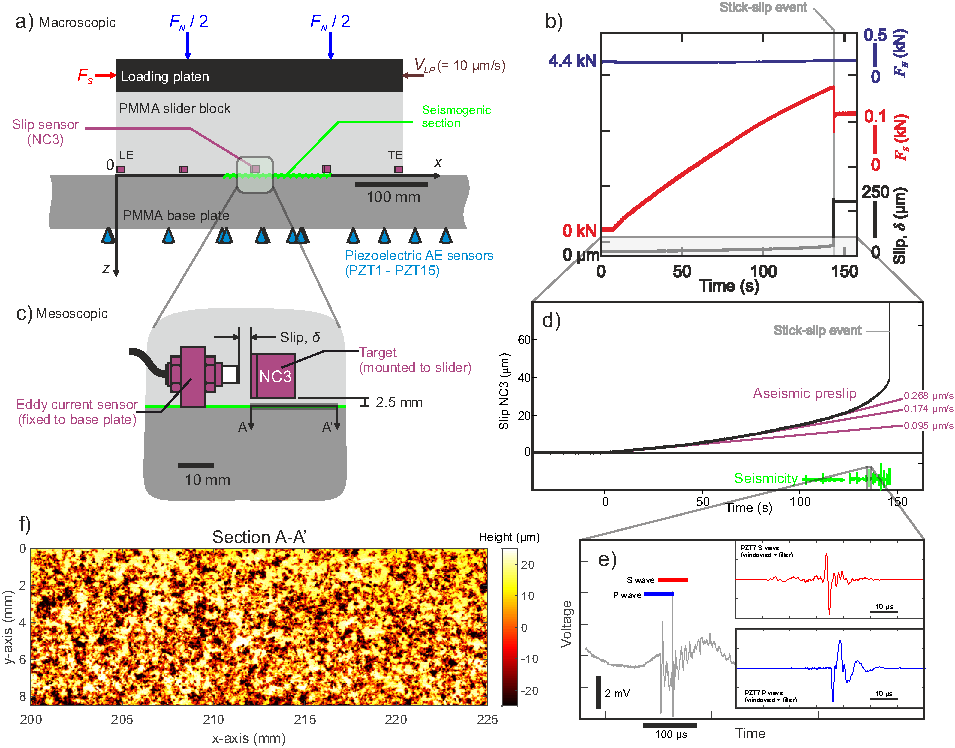
\includegraphics{FIG1.pdf} 
 	\caption{ \textbf{(a)} Schematic details of the direct shear friction apparatus. General loading conditions and sensor placements are shown. For more technical details please consult the literature \cite{Selvadurai2015, Selvadurai2015a}. \textbf{(b)} Typical result demonstrating the bulk frictional evolution in terms of shear slip and shear force leading up to failure. Normal force was constant and the macroscopic loading rate was $V_{LP}$  = 0.010 mm s$^{-1}$; the normal force was fixed at $F_{n}$ = 4400 N. \textbf{(c)} Schematic details of the non-contact eddy current sensor placement at the mesoscopic scale. \textbf{(d)} Detailed slip measurement during the experiment shown in (b).  Mesoscopic slow aseismic slip was observed leading up to macroscopic stick-slip failure.  Lines of constant slip velocity are shown for reference.  Seismicity (green) is represented schematically to show the presence of local fast slip as the accelerated aseismic slip was observed. \textbf{(e)}  An example of precursory seismicity recorded using PZT7.  Seismicity showed clear P and S wave arrivals. More detailed source analysis has been performed by \citeA{Selvadurai2019}. \textbf{(f)} Surface roughness measurement taken \textit{a posteriori} using the longer length scale optical profilometer (Nanovea P50).  The region on the fault associated with this scan is shown by the cross-section A-A’ in (c).}
 	\label{fig1}
 \end{figure}
 
 In Figure \ref{fig1}(b) the slip evolution (black line) for the stick-slip event as measured by the non-contact eddy current sensor (NC3) is shown.  Figure \ref{fig1}(c) depicts a schematic representation of the eddy current sensor (mounted to the base plate) and the wing target attached to the slider block $\sim$ 2.5 mm on above the interface.  The inductive eddy current sensors measured slip $\delta$ in the $x$-direction. We refer to this scale as the mesosopic scale for the discussion.   
 
 During a stick-slip cycle we observe slow and smooth accumulation of aseismic as detailed in Figure \ref{fig1}(d). We show lines of constant slip rate (magenta), which are superimposed over the slip evolution curve.  We see that the fault displayed an acceleration of aseismic slip leading up to the stick-slip event. This type of observation is fairly common in the laboratory friction experiments. However, we also observe pronounced impulsive events detected using the array of absolutely calibrated piezoelectric transducers (PZT) that measure high-frequency vibrations (100kHz to 1500 kHz) produced by stress waves.
 
 In Figure \ref{fig1}(d) seismicity is shown schematically (green) since the time scales between the slow slip and this impulsive source was $\sim$ 6 orders of magnitude different.  Figure \ref{fig1}(e) shows isolated P and S waves from a typical impulsive source as measured by PZT7.  Seismological analysis that employed kinematic point source models based on physics associated with dynamic shear crack \cite<e.g.>[]{Brune1970, Brune1971} were already used to infer source properties for these emissions in a concerted study by \citeA{Selvadurai2019}.
 
As mentioned before, our friction model requires spatial heterogeneity to explain the observations of concomitant  slow (Figure \ref{fig1}(d)) and fast rupture (Figure \ref{fig1}(e)). We base spatial heterogeneity on the experimental \textit{a posteriori} measurement of surface roughness.  Optical profilomerty was performed using two devices that measured longer and shorter length scales with increasing resolution. Figure \ref{fig1}(f) shows the optical scan of the top slider blocks surface through the cross-section A-A' in Figure \ref{fig1}(d).  The scans were taken below the non-contact sensor NC3 as shown.  Details of the metrics used to quantify the surface are given next.  

\section{Characterizing Roughness}

\subsection{Surface Roughness Analysis}
\label{SRA}

Based on the different metrics used to quantify surface roughness in the fields of contact mechanics, tribology and geophysics we will characterize the interfaces using four standard metrics. We deploy a measure of average roughness known as the root mean square:

\begin{equation}
h_{rms} = \sqrt{\left(\frac{1}{N} \right) \sum^{N}_{i=1} h_{i}^{2}} ,
\label{eq99}
\end{equation}

\noindent where $N$ is the total number of points and $h_{i}$ is the individual surface height. To estimate statistical properties of surface heights we also employ the probability density functions (PDFs) of the surface height $h$ defined by a modal Gaussian distribution. Given as follows:

\begin{equation}
\phi(h) = \left( 2\pi \sigma \right) exp\left[ \frac{\left(h - \mu^{*}\right)^{2}} { 2\sigma^{2}}  \right],
\label{eq1}
\end{equation} 

\noindent where $\mu^{*}$ is the arithmetic mean and $\sigma$ is the standard deviation. Building on equation \eqref{eq1} we can also describe the PDF for a bimodal Gaussian mixture model as 

\begin{equation}
\Phi(h) = p\cdot \phi_{1}(h)+\left(1-p\right)\cdot \phi_{2}(h),
\label{eq2}
\end{equation}

\noindent where $p$ is the mixture ratio between the two Gaussian distribution functions $\phi_{1}$ and $\phi_{2}$, each with their individual means and standard deviations. When fitting \eqref{eq1} and \eqref{eq2} to the experimental measurements we employ a maximum likelihood estimation (MLE) of the means, standard deviations and mixture ratio. Finally, we also estimate surface properties using power spectral density (PSD), i.e.  the square of the modulus of the normalized Fourier transform, of a self-affine surface profile following 

\begin{equation}
P(k) \propto k^{-(1+2H)},
\label{eq999}
\end{equation}

\noindent where $k$ is the wavenumber and $H$ is the self-affine scaling exponent or Hurst exponent \cite{Schmittbuhl2003, Candela2009, Mai2002}. The wavenumber $k = 1/\lambda$ where $\lambda$ is wavelength. By plotting equation \eqref{eq999} we can estimate $H$ using linear regression of log-log slope of the relationship between the PSD and wavenumber $\beta =-(1+2H)$.  

A sensitivity analysis was performed by generating two isotropic synthetic surfaces where $H_{input}$ = 0.4 and 0.6 using the algorithm provided by \citeA{Candela2009}.  For each 1-D profile the power spectrum was calculated and PSDs were stacked to reduce the effects of noise.  The estimated Hurst exponents for the synthetic surfaces were $H_{output}$ = 0.45 (3\% error) and 0.65 (8.3\% error), which was deemed to be an acceptable approximation of this approach according to \citeA{Candela2009}.  

%%%%%%%%%%%%%%%%%%%%%%%%%%%%%%%%%%%%%%%%%%%%%%%%%%%%%%%%%%%%%%%%%%%%%%%%%%%%%%%%%%%%%%%%%%%%%%%%%%%%%%%%%%%%%%%%%%%%%%%%%%%%%
\subsection{Surface Roughness of a Worn Interface}
\label{SurfaceRoughnessResults}

Here we employ the methods described in Section \ref{SRA} to quantify the surface characteristics of the slider block. The facilities and measurement techniques are discussed in detail by \citeA{Selvadurai2017}. A Nanovea PS50 optical profilometer was used to measure longer length scale variations in surface height (cm to millimeter), whereas the ADE MicroXAM-100 optical profilometer was used to measure small length scales (sub-millimeter) on the smoother, worn sections of the fault. We consider both measurements to fall on the mesoscopic scale shown in Figure \ref{fig1}(c).

\begin{figure}
	\centering
	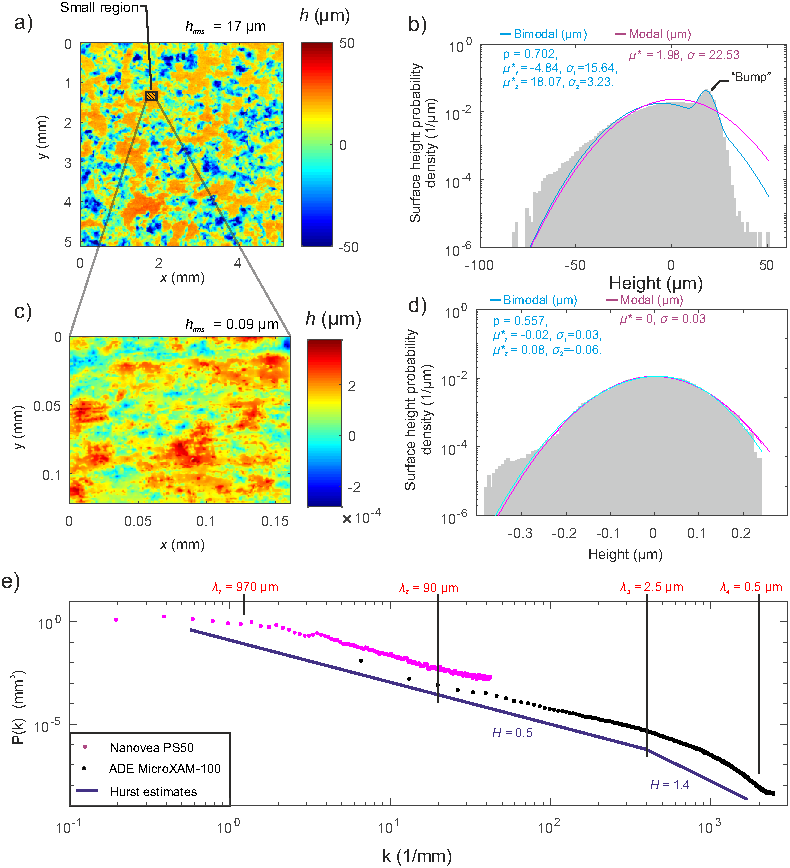
\includegraphics{FIG2.pdf} 
	\caption{\textbf{(a)} Surface roughness for a 5 mm x 4.8 mm section within the seismogenic region taken from Figure \ref{fig1}(f). \textbf{(b)} Surface height probability of the region in (a) and the bimodal (cyan) and modal (purple) Gaussian estimates are shown. We note the pronounced ``bump'' in the right-hand tail that is a manifestation of wearing processes. \textbf{(c)} Surface roughness of a random smooth section within the seismogenic region of the fault. \textbf{(d)} Surface height probability of the region in (c) is shown with the bimodal (cyan) and modal (purple) Gaussian estimates. \textbf{(e)}  Power spectral density of the surface roughness of both the ADE MicroXAM-100 and Nanovea PS50 optical profilometer. }
	\label{fig2}
\end{figure}

In Figure \ref{fig2}(a) we show a 5 mm x 4.8 mm section of height measurements taken from the seismogenic region of the fault. The spatial resolution of the Nanovea P50 was 10 $\mu$m.  Within this region the root mean square roughness was $h_{rms}$ = 17 $\mu$m. In Figure \ref{fig2}(b) we examine the surface height probabilities using equations \eqref{eq1} and \eqref{eq2}.

We note a distinct ``bump'' in the surface height probability density that was due to wear.  It is apparent that the standard modal Gaussian distribution of height probability does not characterize this surface adequately at this length scale. The bimodal estimate of roughness is reasonable for surface height probabilities $>$ 10$^{-2}$ = 0.01 (1\%). The maximum and minimum wavelength considered using the long length scale scans were $\lambda_{1} = 1/k_{1} =$  0.90 mm and $\lambda_{2} = 1/k_{2}=$ 0.09 mm. The sensitivity of $H$ is due to the ``roll-off'' at wavelengths greater than $\sim$1 mm likely due to the limited size of our experimental measurements. 

To extend our understanding to smaller length scales we used the ADE MicroXAM-100 optical profilometer. All scans using this profilometer targeted the flat, worn sections that contributed to the ``bump'' in the surface height probabilities.  A Gaussian window of 2 pixels ($\sim$ 0.2 $\mu$m) was convolved with the scans to remove any experimental errors at lower spatial length scales \cite{Candela2009}.  A total of 40 scans were taken on these flat sections and an average root mean square roughness was $h_{rms}$ = 0.09 $\mu$m  -- approximately 188 times smoother than the larger section by this metric.  In Figure \ref{fig2}(c) we show a typical scan of the flat region (0.128 mm x 0.0975 mm).    Figure \ref{fig2}(d) shows the accompanying surface height probability density along with the Gaussian modal (magenta) and bimodal (cyan) surface height probability distribution estimates.  We note that the improvement of the bimodal model is not as significant at the smaller scale. The values of the means ($\mu^{*}$), standard deviations ($\sigma$) and mixture ratio ($p$) are shown for the modal (magenta) and bimodal (cyan) models with units of $\mu$m.

In Figure \ref{fig2}(e) we plot the PSD of the long wavelength measurements using the Nanovea PS50 (purple, see also Figure \ref{fig2}(c)) along with the new, shorter wavelength PSD measurements obtained from the ADE MicroXAM-100 scans (black dots).  Between $\lambda_{1}$ and $\lambda_{2}$, we show our estimate of the Hurst exponent $H = $ 0.46 $\pm$ 0.02.  Estimating the Hurst exponent below $\lambda_{2}$ is more complicated since the PSD estimate at shorter wavelengths does not show a clear linear log-log behavior as before.  Two estimates of the Hurst exponent $H$ = 0.5 and 1.4 are shown for reference.  

%%%%%%%%%%%%%%%%%%%%%%%%%%%%%%%%%%%%%%%%%%%%%%%%%%%%%%%%%%%%%%%%%%%%%%%%%%%%%%%%%%%%%%%%%%%%%%%%%%%%%%%%%%%%%%%%%%%%%%%%%%%%%
\section{Rate- and state-dependent (RSF) friction model}
\subsection{Theory}
\label{Theory}

In this section we develop a RSF model to help understanding the complex frictional behavior shown in Figure \ref{fig1}.  RSF constitutive friction law is phenomenological and derived from laboratory experiments \cite{Dieterich1979}.  The model describes the behavior of a faults resistance to sliding in terms of the shear stress $\tau$ as a function of the slip rate $V$ and a state variable $\theta$. This is given as:

\begin{equation}
\label{eq5}
\tau \left( V,\theta \right) = \sigma \left[\mu^{*} + a \ln\frac{V}{V^{*}} + b \ln\frac{V^{*}\theta}{D_{c}}\right],
\end{equation}   

\noindent where $\sigma$ is the effective normal stress, $\mu^{*}$ is the reference steady-state friction coefficient at an arbitrary reference slip rate $V^{*}$, $D_{c}$ is the characteristic slip distance and, $a$ and $b$ are constitutive parameters describing the direct and evolution effects, respectively.  The state parameter in our study is referred to as the so-called ``slip law’’ and is adopted due to its ability to model recent laboratory studies \cite{Bhattacharya2015, Kaneko2011, Kaneko2016}:

\begin{equation}
\label{eq6}
\dot{\theta} = - \frac{V\theta}{D_{c}}\ln\frac{V\theta}{D_{c}},
\end{equation}   

\noindent where friction at steady state ($\dot{\theta} $ = 0) is given as

\begin{equation}
\label{eq7}
\tau_{ss} \left( V \right) = \sigma \left[\mu^{*} + \left(a - b \right)\ln\frac{V}{V^{*}}\right].
\end{equation}   

\noindent From equation \eqref{eq7} we see that constitutive parameters $\left(a - b \right)$ play an influential role as to how the interface behaves at steady-state.  For $\left(a - b \right) < 0$, $\tau_{ss}$ will decrease as slip rate $V$ increases.  A fault with these characteristics is known as velocity-weakening (VW) and is prone to spontaneous instability if the fault stiffness is below a critical stiffness. Stiffness of the VW spring-slider system was investigated by \citeA{Ranjith1999} who found the critical stiffness to be:

\begin{equation}
\label{eq9}
k_{cr}=\frac{\sigma \left( b-a \right)}{D_{c}},
\end{equation}   

\noindent where $\sigma$ is the (effective) normal stress on the fault. This implies that quasi-static steady-state slip is stable ($V \rightarrow V^{*}$) or unstable ($V \rightarrow \infty$) as the spring stiffness is greater than or less than the critical value $k_{cr}$, respectively. Fault stiffness is inversely proportional to the minimum half-length of a nucleation zone capable of instability:

\begin{equation}
\label{eq8}
L_{c} = \eta \frac{G^{*} D_{c}}{ \sigma \left( b-a\right)},
\end{equation}   

\noindent where $\eta = (7\sqrt{2})/(3\pi)$ \cite{Dieterich1992} for a square patch, the corrected shear modulus $G^{*} (= G/(1-\nu))$ was employed due to the Mode II plane strain conditions and $\nu$ is the Poisson's ratio. 

The equation of motion controlling slip on a planar fault in our model is given by:

\begin{equation}
\label{eq8a}
\tau_{el}\left( \mathbf{x} \right) - \tau\left( \mathbf{x} \right) = \frac{G^{*}}{2 V_{S}} V(\mathbf{x}),
\end{equation}  

\noindent where $\tau_{el}$ is defined as the elastostatic shear stress due to the loading boundary condition \cite{Horowitz1989}. The inertial term on the right hand side represents the radiation damping term for S waves produced along the fault at point $\mathbf{x}$, which propagated with a shear wave speed $V_{S}$ \cite{Rice1993}. Quasi-static interactions between fault elements are calculated using the boundary element method (BEM) and all calculations reported in this study was solved using a Quasi-DYNamic earthquake simulator \cite{Luo2017}. QDYN is a boundary element software to simulate earthquake cycles (seismic and aseismic slip on tectonic faults) under the quasi-dynamic approximation (quasi-static elasticity combined with radiation damping) on faults governed by RSF and embedded in elastic media.  Solution convergence and mesh discretization of the heterogeneous models described later is given in Supplemental Methods S1.

From derivations by \citeA{Dieterich1992} we know that RSF combined with elasticity leads to the common length scale

\begin{equation}
\label{eq8b}
L_{b} \equiv \frac{G^{*}D_{c}}{\sigma b}.
\end{equation}  

\noindent This characteristic dimension was later theoretically confirmed by \citeA{Rubin2005} and controls aspects of earthquake nucleation and the transition from aseismic to seismic behaviour. We define this transition threshold to be:

\begin{equation}
\label{eq8c}
V_{dyn} = \frac{2 a V_{s}}{G^{*}},
\end{equation}  

\noindent which represents the transition point where the inertial term in equation \eqref{eq8a} becomes significant. 

%%%%%%%%%%%%%%%%%%%%%%%%%%%%%%%%%%%%%%%%%%%%%%%%%%%%%%%%%%%%%%%%%%%%%%%%%%%%%%%%%%%%%%%%%%%%%%%%%%%%%%%%%%%%%%%%%%%%%%%%%%%%%
\subsection{Recent advances RSF modelling in the laboratory}

\citeA{Dieterich1994a} showed that the RSF phenomenological behavior holds for various frictional surfaces on a range of materials (granite, soda-lime glass, Lucite plastic and wood among others).  Extensive work has shown that this constitutive model also holds for gouge filled interfaces \cite<see review by>[]{Marone1998}.  The typical manner used to extract constitute parameters $a$, $b$ and $D_{c}$ is performing shearing experiments where constitutive equations \eqref{eq5} and \eqref{eq6} are fitted to bulk (macroscopic) measurement of friction ($\mu = F_{s}/F_{n}$) while performing step-changes in the driving velocity ($V_{LP}$).

Experiments performed by \citeA{Nielsen2010} and \citeA{Latour2013} have benefited from increasing the faults compliance by using analog materials (glassy polymers) in frictional tests. In these experiments, improved spatio-temporal measurement of slip was achieved by using high speed digital cameras. Increased refinement in both spatial and temporal measurements clearly showed the so-called ``preslip'' or nucleation zone.  This nucleation region was predicted in RS models \cite{Dieterich1992, Rubin2005, Ampuero2008} but was difficult to show definitively before novel sensing techniques.

Modelling efforts by \citeA{Kaneko2011} and \citeA{Kaneko2016} have shown that frictional behavior of the `plastic-on-plastic' sliding experiments can be explained using RS friction models. These models are informative and promote the idea of a `smooth transition' of frictional sliding over the macroscopic length scale of the experimental fault. It explained both the spatial and temporal evolution of observed nucleation features of those laboratory ruptures. Similarly, we also observe a breakout style of rupture at the macroscopic scale. In Figure \ref{fig1}(d) this same smooth quasi-static evolution of slip is present. However, we benefit from additional phenomenological insight. The dynamic piezoelectric (PZT) sensors were able to detect and isolate local instabilities in the same regions experiencing macro-slow slip (Figure \ref{fig1}(e)).  To explain these instabilities in the RS framework we need to investigate the type of heterogeneity at a scale below one the dictates the smoother macroscopic behavior.

Roughness induces complex frictional behavior due to the deviation of a fault from planarity.  This is believed to impose strong effects on many aspects of the earthquake cycle.  Roughness appears to influence the static deformation at large scales \cite<e.g.>[]{King1985}, dynamic rupture propagation \cite<e.g.>[]{Dunham2011, Fang2013, Mai2018}, nucleation physics \cite<e.g.>[]{Tal2018} and the presence aseismic transients \cite{Ozawa2019}. The studies conducted by \citeA{Tal2018} and \citeA{Ozawa2019} show that RSF in combination of the non-planarity of the fault can help to understand the presence of asymmetric nucleation zones, non-monotonic increase in slip rates and the generation of multiple slip pulse that self-arrests. Most studies that incorporate both RSF and roughness assume mated initial fractures as initial conditions. They predominantly characterize surface topography using the Hurst exponent in equation \eqref{eq999}.  In our study we deviate from the initial condition of perfect matedness in the other studies. We choose to instead create a range of 1-D models with attributes derived from the spatial complexity of the measured roughness profile that exhibited signs of wear.  As the level of matedness of the surfaces was unclear at any time in the experiment, we chose to use a roughness \textit{cutting plane method} that is able to separate the two modal Gaussian distributions of roughness in space.

%%%%%%%%%%%%%%%%%%%%%%%%%%%%%%%%%%%%%%%%%%%%%%%%%%%%%%%%%%%%%%%%%%%%%%%%%%%%%%%%%%%%%%%%%%%%%%%%%%%%%%%%%%%%%%%%%%%%%%%%%%%%%
\subsection{Cutting plane method}

The \textit{cutting plane method} splits the roughness into two separate sections: smooth and rough. Using this method we assign two sets of frictional parameters to the smooth (upper) and rough (lower) regions of the roughness profile that appeared due to wear, which will be the input to our numerical rate and state model. A `cutting plane' was defined to be exactly between the two means of the bimodal distributions that formed due to wear. While this method could be extended to 2-D, in this study we build a simple 1-D model and choose arbitrarily the transect of rough surface at $y$ = 2 mm. Figure \ref{fig3}(a) shows the roughness along $x$ at $y$= 2 mm (black line).  This transect is taken from a highly seismogenic section of the interface \cite{Selvadurai2015}. 

The cutting plane (red) was defined as $h_{cut} = \left(\mu^{*}_{1}+\mu^{*}_{2} \right)/2$ = 6.6 $\mu$m.  Figure \ref{fig3}(b) shows the probability distribution of the surface heights from the sample transect and the cutting plane in red. We assume that the top surface is relatively ``smooth'' from the preferential wearing of asperity tops and bottom surface, as is described in more detail in Section \ref{SurfaceRoughnessResults}.

\begin{figure}[ht]
	\centering
	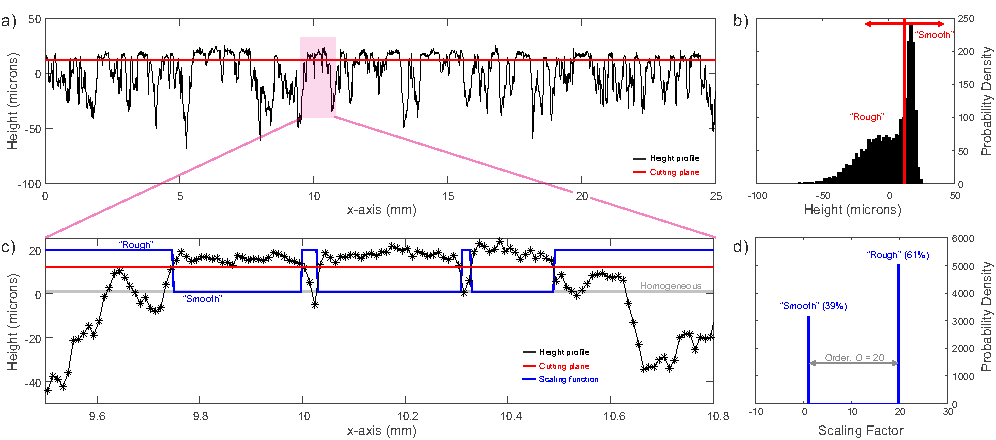
\includegraphics{FIG3.pdf} 
	\caption{ \textbf{(a)} 1-D roughness profile (black) taken from the transect at $y$ = 2 mm in Figure \ref{fig1}(f).  The cutting plane $h_{cut}$ = 6.6 $\mu$m is used to separate the bimodal distribution into smooth and rough surfaces. \textbf{(b)} PDF of the height profile in (a) with the cutting plane shown. \textbf{(c)} Small section of the height distribution showing the roughness profile (black line), the cutting plane (red line) and the scaling function (blue line). \textbf{(d)} PDF of the scaling function $\mathrm{SF}(x)$ with an order of heterogeneity $O$ = 20.}
	\label{fig3}
\end{figure}

A scaling function (\textit{SF}) is used to partition the smooth and rough sections of the fault. Figure \ref{fig3}(c) shows a detailed view of the roughness (black), the cutting plane (red) and the scaling function (blue). When the roughness was above the cutting plane we defined a scaling function (\textit{SF}) to have value of unity. All heights below the cutting plane were prescribed as scaled value. This allowed us to control the magnitude of heterogeneity we call the `order'. For this example the order was $O$ = 20. The SF produced heterogeneity in two manners: (\textit{i}) spatial variations were controlled by the location where the roughness profile crossed the cutting plane and ($ii$) the level (order) of heterogeneity -- the peak-to-peak range of \textit{SF} -- could be prescribed by the modeler. The order of the SF is seen more clearly in probability distribution function in Figure \ref{fig3}(d).

	The basis for the cutting plane was to separate the interface into the two predominant rough and smooth surfaces, that we believe, existed due to wear.  Micromechanical simulations performed by \citeA{Yoshioka1996} showed that $D_{c}$ decreases as faults become smoother in dry, gouge-free scenarios such as in our experimental conditions. We  note that smoother surfaces likely produced locations capable of supporting higher localized patches of normal stress. From equation \eqref{eq8} we see that a combination of high $\sigma$ and low $D_{c}$ might be a viable mechanism for the initiation of localized seismicity. This will be examined using a range of 1-D RS models developed next.

%%%%%%%%%%%%%%%%%%%%%%%%%%%%%%%%%%%%%%%%%%%%%%%%%%%%%%%%%%%%%%%%%%%%%%%%%%%%%%%%%%%%%%%%%%%%%%%%%%%%%%%%%%%%%%%%%%%%%%%%%%%%%
\subsection{Frictional parameter space}
\label{ParameterSpace}

It is important to know that we are choosing parameters that are based on previous studies surrounding this experiment but also incorporate assumptions from the literature. The goal of the models is to identify conditions that may produce local seismicity -- a critical experimental observation made from the PZT sensors. In Figure \ref{fig4} we investigate how the critical nucleation length $L_{c}$ (equation \eqref{eq8}) varies with $D_{c}$ and the normal stress $\sigma$.  Based on experiments performed by \citeA{Berthoude1999} we set $a/b$ = 0.65 and $b$ = 0.0144. Curves representing constant critical nucleation length are shown in red for $L_{c}$ = 25 mm and 0.9 mm, for reference.   

\begin{figure}
	\centering
	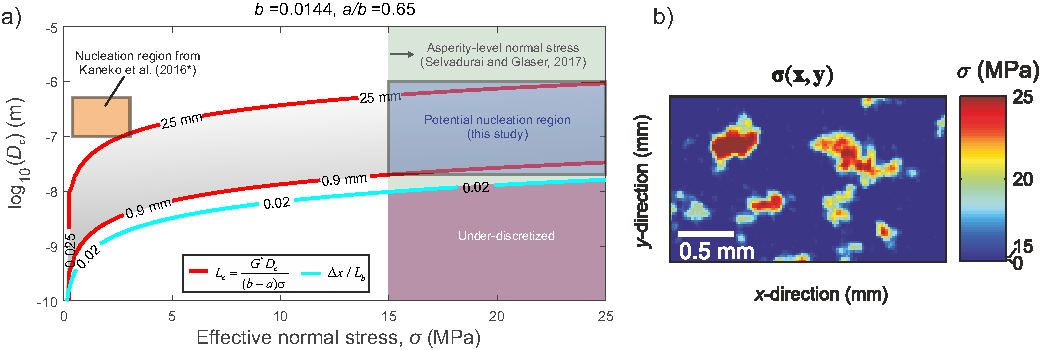
\includegraphics[scale = 0.95]{FIG4.pdf} 
	\caption{(a) Initial estimates of the nucleation parameter space ($L_{c}$) based on measurements of local normal stress \cite{Selvadurai2017}, minimum mesh discretization ($\Delta x /L_{b}$) and maximum critical nucleation size $L_{c} = 0.025$ m. The gray hatched region represents possible nucleation sizes for the mesoscopic length scale.  The hatched orange shows the ranges of $D_{c}$ and effective normal stress $\sigma$ that nucleated gross fault in \citeA<>[, *$a/b$ = 0.6944]{Kaneko2016}. (b) Example of asperity-level normal stress field measured using an experimental pressure sensitive film (adapted from \citeA{Selvadurai2017}.)}
	\label{fig4}
\end{figure}

To further constrain our models, we examined the experimentally measured asperity normal stress from the concerted study by \citeA{Selvadurai2017}. Using the calibrated pressure film \cite{Selvadurai2015}, they found the asperities attained normal stresses ranging from $\sigma$ = 12 to 25 MPa. This range of normal stress is superimposed in Figure \ref{fig4}, which further bounds the potential nucleation conditions in the RSF model.  The goal in our study was to better constrain our numerical models using a wide variety of measurements made at a mesoscopic scale.  By constraining the parameterization we can also better understand numerical requirements.  

Finally, it was necessary to ensure that the fault was properly meshed to correctly capture the dynamic processes at the rupture tip during seismic events. Our calculations were based on the estimates of the cohesive (or breakdown) zone length scale $L_{b}$ in equation \eqref{eq8b}. To accurately capture local frictional breakdown it was necessary to apply a minimum grid size of $\Delta x/L_{b} <$ (1/50), which for $a/b$ = 0.65 was deemed acceptable.  In this model we choose to use 2$^{13}$ = 8192 grid points over the length $L$ = 25 mm of the mesoscopic domain, resulting in a resolution $\Delta x \sim$  3 $\mu$m. This is much different that the macroscopic parameter space estimated by \citeA{Kaneko2016}, shown as orange hatched region, for the plastic-on-plastic sliding experiment performed by \citeA{Latour2013}. Table \ref{table1} shows the baseline frictional, material and length scale properties used in this study. More information on the convergence tests for the heterogeneous models (discussed later) is given in the Supplemental Information S1. A summary of the parameters used to develop the homogeneous and later heterogeneous models are given in Table \ref{table1}.

\begin{table}[ht]
	\centering
	\caption{General model Parameters used in the 1-D RS mesoscopic models.}
	\begin{tabular}{ m{5cm} m{2cm} m{4cm}} 
		\hline  
		\bf{Parameter} 			& \bf{Symbol} 		& \bf{Value}	\\
		Shear modulus  			& $G$  		 	& 2.39 GPa		\\
		Poisson ratio  			& $\nu$  	 	& 0.32 		\\
		Shear wave speed		& $V_{S}$      		& 1330 m s$^{-1}$	\\
		Reference friction coefficient	& $\mu^{*}$	        & 0.6	\\
		Reference slip rate  		& $V^{*}$     		&  0.1 $\mu$m s$^{-1}$\\
		Dynamic sliding threshold   	& $V_{dyn}$  		& 0.177 m s$^{-1}$ \\
		Loading plate velocity  	& $V_{LP}$     		&  0.1 $\mu$m s$^{-1}$\\
		Lower critical slip distance 	& $\left(D_{c}\right)_{low}$    &  25 nm\\
		Normal stress 			& $\sigma$  		&  25 MPa \\
		Length of mesoscopic domain 	&   $L$  		& 25 mm\\
		Height of mesoscopic domain 	&   $H$  		& 2.5 mm\\
		Width of mesoscopic domain 	&   $W$   		& $\infty$\\
		Grid size 			& $\Delta x$ 		& 3 $\mu$m \\
		Grid points 			& $n$ 			& 2$^{13}$ \\
		RS parameter $b$ (VW)  		& $b$ 			& 0.0144  \\
		RS parameter $a$ (VW)  		& $a$ 			& 0.00936  \\
	    Simulation time 			& $t_{sim}$ 		& 600 s  \\
		\hline  	
	\end{tabular}
	\label{table1}
\end{table}

%%%%%%%%%%%%%%%%%%%%%%%%%%%%%%%%%%%%%%%%%%%%%%%%%%%%%%%%%%%%%%%%%%%%%%%%%%%%%%%%%%%%%%%%%%%%%%%%%%%%%%%%%%%%%%%%%%%%%%%%%%%%%
\section{Computational Results}

The general domain for the 1-D frictional model is shown in Figure \ref{fig5}(a). This represents the small region of material under the eddy current target shown in Figure \ref{fig1}(c). The geometry of the domain is $L$ = 25 mm (corresponding to the extent of the roughness measurement in the direction of slip), $H$ = 2.5 mm (corresponding to the height of the material just below the eddy current target) and $W$ = $\infty$ (corresponding to plane strain conditions). The boundary element code QDYN assumes frictional properties ($a$, $b$ and $D_{c}$) and normal stress ($\sigma$) at each node on the interface. The models behavior is described in Section \ref{Theory}. Figure \ref{fig5}(b) shows a schematic representation of the boundary value problem. A few representative nodes are shown as blocks. Communication between the frictional nodes is shown as spring elements. This interaction is solved by QDYN  and the spring constants are defined in equation \eqref{eq9} equation of motion controlling slip on a planar fault. Before moving to more complex, heterogeneous cases we examine the behavior of the homogeneous case to develop a baseline.    

%%%%%%%%%%%%%%%%%%%%%%%%%%%%%%%%%%%%%%%%%%%%%%%%%%%%%%%%%%%%%%%%%%%%%%%%%%%%%%%%%%%%%%%%%%%%%%%%%%%%%%%%%%%%%%%%%%%%%%%%%%%%%
\subsection{Homogeneous case}

From the mesoscopic geometry we build the 1-D homogeneous model, shown schematically in Figure \ref{fig5}(b). For the homogeneous case, each node has velocity-weakening (VW) conditions ($a-b$) = -0.005, $a/b$ = 0.65, normal stress $\sigma$ = 25 MPa and a critical slip-weakening distance $D_{c}$ = 25 nm. For the homogeneous case, the steady-state sliding velocity $V^{*}$ was assumed to be equal to the load point velocity $V_{LP}$. We were able to determine this experimentally from the near-fault slip velocity measurements made using the eddy current slip sensors shown in Figure \ref{fig1}(d). $V_{LP}$ = 0.1 $\mu$m/s.

\begin{figure}
	\centering
	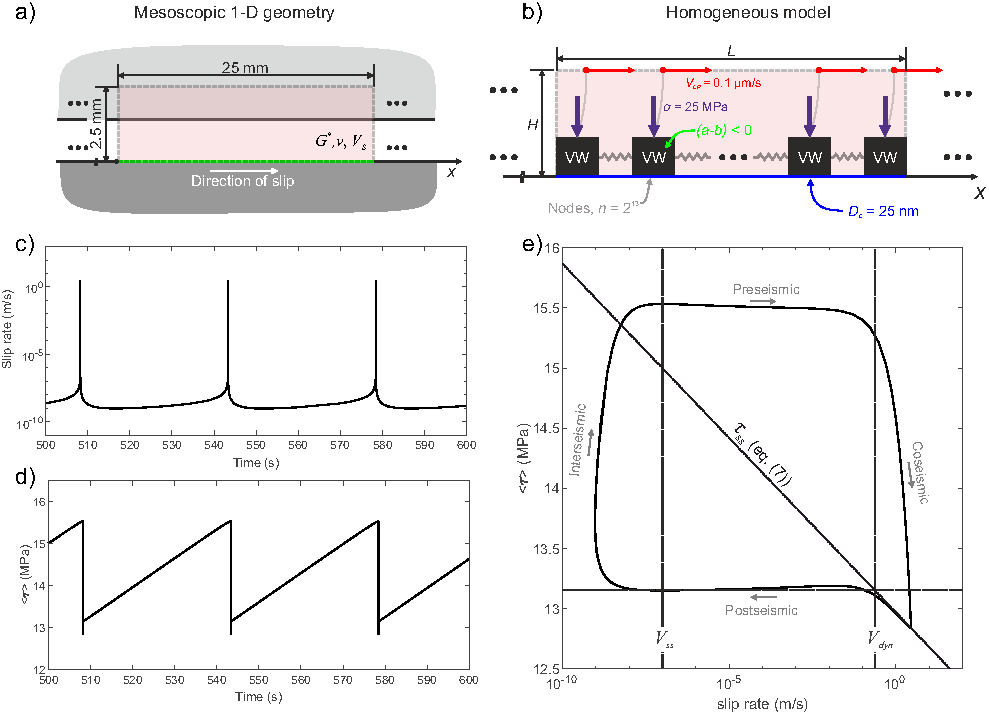
\includegraphics{FIG5.pdf} 
	\caption{\textbf{(a)} General dimensions of the model domain described in Figure \ref{fig1}(c). \textbf{(b)} Description of the 1-D boundary value problem being solved by QDYN.  RS frictional behavior is described by equations \eqref{eq5} to \eqref{eq8}. \textbf{(c)} Average slip velocity and \textbf{(d)} average shear stress along the fault between $t_{sim}$ between 500 to 600s. We see that the fault underwent stick-slip behavior. \textbf{(e)} A diagram of the earthquake cycle for the VW fault that includes preseismic, coseismic, postseismic and interseismic phases.}
	\label{fig5}
\end{figure}

Each numerical simulation lasted for $t_{sim}$ = 600 s, which allowed for the fault to fully-develop a periodic stick-slip response \cite{Hillers2007}.  Figure \ref{fig5}(c) and (d) shows a small time window (500 to 600 s) of the slip velocity and shear stress, respectively, averaged over all nodes in the model.  We see that periodic ruptures are analogous to a `stick-slip' event \cite{Scholz2002}. Over the full simulation, 18 stick-slip were recorded for the homogeneous case but only three are shown here.  Coseismic slip was defined when any node experienced a sliding velocity $V > V_{dyn}=$0.177 m/s as determined from equation \eqref{eq8c}. To further characterize the homogeneous case, Figure \ref{fig5}(e) shows the relationship between average slip velocity and shear stress. We find a similar behavior as the modelling exercise performed by\citeA{Ampuero2008} in that the fault moves through the interseismic, preseismic, coseismic and postseismic regime.

%%%%%%%%%%%%%%%%%%%%%%%%%%%%%%%%%%%%%%%%%%%%%%%%%%%%%%%%%%%%%%%%%%%%%%%%%%%%%%%%%%%%%%%%%%%%%%%%%%%%%%%%%%%%%%%%%%%%%%%%%%%%%
\subsection{Heterogeneous $D_{c}$-model}

We produce heterogeneity by varying the critical slip weakening distance $D_{c}$ according to the scaling function (SF) in Figure \ref{fig3}(c). The $D_{c}$-model shares some properties of the homogeneous case ($b$ = 0.0144, $a/b$ = 0.65, $\sigma$ = 25 MPa) and is depicted schematically in Figure \ref{fig6}(a).  However, the main distinction arises from the non-uniform distribution of the critical slip distance. For the $D_{c}$-model we prescribe the lower value of critical slip weakening distance $(D_{c})_{low}$ = 25 nm. Using the scaling function from the cutting plane method, we can capture the spatial variation in critical slip weakening distance given as $D_{c}(x) = (D_{c})_{low} \cdot \mathrm{SF}(x)$. Figure \ref{fig6}(b) shows the spatial fluctuations in $D_{c}(x)$ for heterogeneity on the order of O20. Spatial distribution of the homogeneous properties is shown in Figure \ref{fig6}(c) for reference.
 
The average slip rate and shear stress for this $D_{c}$-model (O20, blue) is shown in blue in Figures \ref{fig6}(d) and (e), respectively. For reference, we also show the results from the homogeneous model O1 (black). We see that the fault does experience some stick-slip behavior -- the small spikes in slip velocity -- but it does not experience full ruptures with large levels of shear stress drop that occurred in the homogeneous case. 

 \begin{figure}
	\centering
	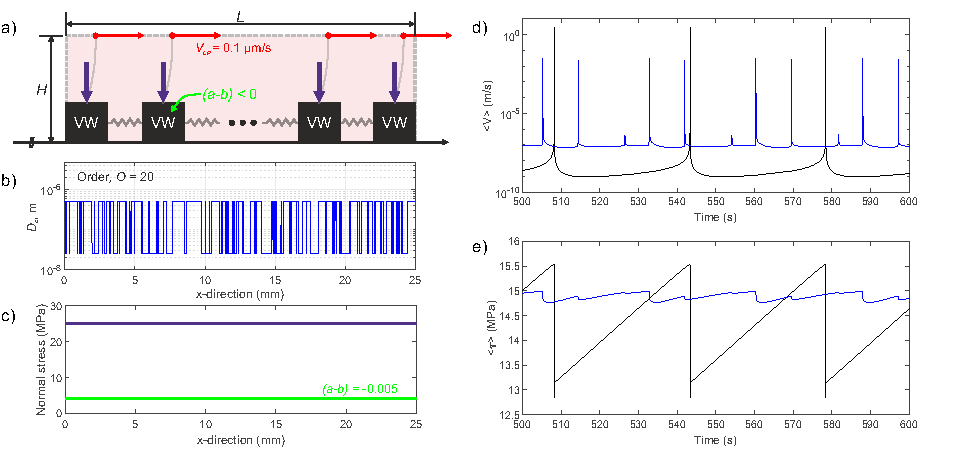
\includegraphics{FIG6.pdf} 
	\caption{\textbf{(a)} General schematic showing the heterogeneous model. \textbf{(b)} Heterogeneous distribution of $D_{c}$, with O20. \textbf{(c)} Constant normal stress and VW rheology ($a-b <$ 0) is shown along the x-axis.  \textbf{(d)} Average slip velocity is shown along the fault for the heterogeneous model (blue line), which is compared to homogeneous model (black line). \textbf{(e)} Average shear stress along the heterogeneous and homogeneous models.}
	\label{fig6}
\end{figure}
 
We investigated the effect of different levels of heterogeneity. In Figure \ref{fig7} the average fault behavior is shown for three levels O10 (red), O15 (green) and O20 (blue), which all use the same scaling function $\mathrm{SF}(x)$.  This is again compared to the average behavior of the homogeneous fault O1 (black).  The average slip, slip rate and shear stress is given in Figures \ref{fig7}(a), (b) and (c), respectively.  We observe an increase in complexity from homogeneity with these models. The first major note is that both O10 (red) and O15 (green) still experienced full system wide rupture (large events that propagated the full extent of the modelled fault).  Full rupture would nucleate from a smooth section of the fault and would not arrest in comparison to more localized ruptures that occurred in the O20, which had stronger barriers. 

While the system wide events did occur on the O10 (red) and O15 (green) faults, they also experienced small localized events that were arrested by the neighbouring barriers. These were denoted as small ``foreshock sequences'' leading up to the main rupture (larger stress drop), which highlighted in Figure \ref{fig7}(c). These foreshock sequences might be similar to experimentally observed detachment fronts that have been routinely observed in frictional experiments \cite<e.g.>[]{Rubinstein2004, Maegawa2010, Kammer2012, Selvadurai2017}.  We clearly see that as the order $O$ is increased, the fault exhibits transition from well-behaved fault (homogeneous, O1) to relatively chaotic mixture of system wide events with small localised ruptures (O10 and O15), then returning to well-behaved creep-dominated fault with small localized events on a preferential patch (O20).

\begin{figure}
	\centering
	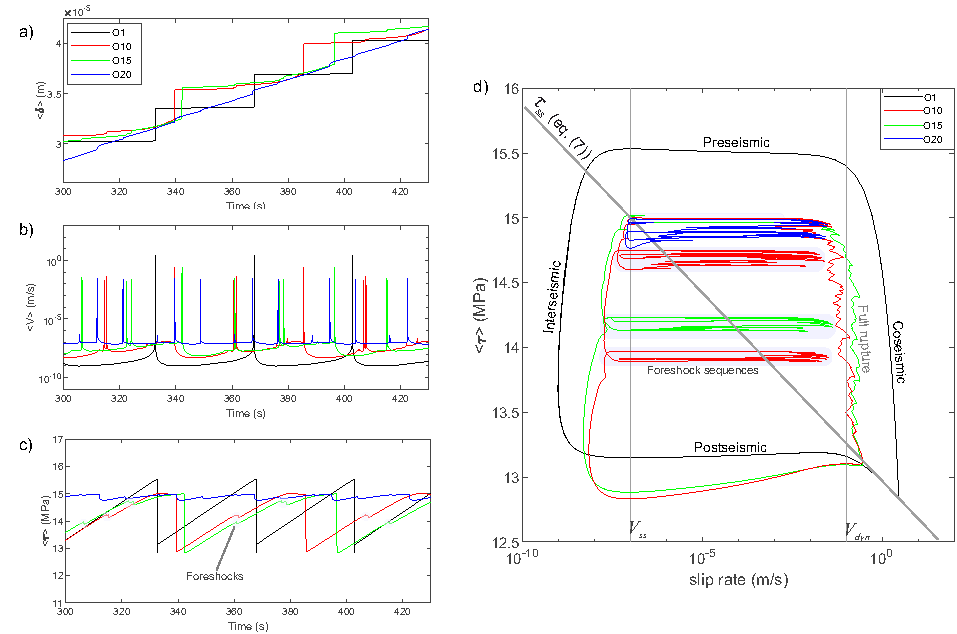
\includegraphics{FIG7.pdf} 
	\caption{Three heterogeneous models $O$ =  10 (red), 20 (green) and 30 (blue) are compared to the homogeneous model (black) for a short time window between 300 and 430 s. We show the \textbf{(a)} average slip, \textbf{(b)} average slip velocity and \textbf{(c)} average shear stress.  We highlight where small drops in shear stress were seen and relate them small localized events (foreshocks). \textbf{(d)} We examine the phase diagram between shear stress and slip velocity for each heterogeneous model in comparison to the homogeneous model.}
	\label{fig7}
\end{figure} 

To better visualize the systems behavior, we plot all models on phase-diagrams described in Figure \ref{fig5}(e) for the homogeneous case. The average fault behavior cycles from co- to post- to inter- to pre-seismic, moving around $\tau_{ss}$ given in equation \eqref{eq7}. With regards to the full cyclical behavior of the fault, the O10 (red) and O15 (green) $D_{c}$-models appear to observe, in general, lower total stress drop during the full rupture events when compared to the homogeneous case.  We also see that during these full ruptures, the average slip rate on these faults is in general lower than the homogeneous case.  For the most heterogeneous fault with order O20, we see that full rupture events did not occur but there was some deviation from steady state caused by small foreshock sequences that deterred the fault from simply `creeping' along at the steady state shear stress. Foreshock sequences appeared in all models and were due to a relatively large `smooth' section of fault determined from the cutting place method. We see these foreshock sequences highlighted in the phase diagram (gray regions). Two major sequences were observed for the O10 and O15 models. Timing of these foreshock sequences, relative to the full fault cycle, are shown for O10(red) in the interseismic stages of the larger rupture cycle. For O15(green), one foreshock sequence occurred in the interseismic portion and one closely after the fault entered the nucleation phase of the larger rupture cycle. As for O20 (blue), this smooth section of the fault prone to localized rupture behaved in a relative synchronous manner. More details to the spatio-temporal complexity of these ruptures are given in the next section. 

%%%%%%%%%%%%%%%%%%%%%%%%%%%%%%%%%%%%%%%%%%%%%%%%%%%%%%%%%%%%%%%%%%%%%%%%%%%%%%%%%%%%%%%%%%%%%%%%%%%%%%%%%%%%%%%%%%%%%%%%%%%%%
\subsubsection{Spatio-temporal behavior}
\label{spatialmodel}

In Figure \ref{fig8} we examine the spatio-temporal evolution of the $D_{c}$-model with O17.5. We note that this model was not presented in the previous section. The purpose of the previous section was to highlight changes in the general fault behavior at three levels of heterogeneity  with distinctly different behavior.

Figure \ref{fig8}(a) shows the spatio-temporal evolution of slip along the fault from time $t$ = 300 s to 600 s. The time step between each isochron was uniform, taken every 30 intervals of adaptive time steps.  We note that if any point on the fault slipped rapidly, the adaptive time step would decrease to accurately solve the boundary value problem. This lead to higher sampling rates when slip velocities increased and decreased time steps were necessary to capture the complex slip behavior during localized seismicity.  Seismicity (red slip isochrones) was defined as any node in the model experiencing slip velocities $V > V_{dyn}=$0.177 m/s. Below this threshold the fault was assumed to be sliding aseismically (blue slip isochrones). Using this description we were able to clearly see the seismic patches.

One such patch is highlighted in Figure \ref{fig8}(a) and enhanced in (c) where we examine slip on the transect $x$ = 5 to 8 mm from $t$ = 300 s to 305 s.  This asperity section of the fault was prone to seismicity in all models, even the O20 that showed limited localized seismicity. Figure \ref{fig8}(b) shows the spatial variability in heterogeneity in $D_{c}$ along that section (for this case with O17.5). In Figure \ref{fig8}(c), we see that the fault actually has blue lines that delineate the seismicity over these five seconds.  This indicates that slip rates drop to below 0.1 m/s allowing us to separate the events into a sequence.  Four individual ruptures are shown.  We note that these events exhibit typical circular crack-like behavior but are still very complex due to both the spatial variability in $D_{c}$, the level of heterogeneity (O17.5) and the continuously evolving shear stress on the fault.  

In Figures \ref{fig8}(d) and (e) we investigate the space-time plot of slip velocity and shear stress, respectively, for Event 4 in the asperity failure sequence. The portion of the fault is shown ($x$ = 5 to 8 mm) and we have superimposed the heterogeneity from (b) for clarity.  We study this rupture in terms of its transition to rapid sliding, how the rupture grows and why it arrests. By modelling ruptures that generate seismicity, we can compare these source features to the ones modelled from an entirely different standpoint, i.e. the seismic waves \cite{Selvadurai2019}. We see that Event 4 nucleates at the edge of a `smooth-rough' boundary ($x \sim$ 7.25 mm) depicted as the purple star. As the rupture expands, it propagates bi-laterally at different rates. We have superimposed three lines of constant velocity 0.5$\cdot V_{S}$ (green), $V_{S}$ (red) and $V_{P}$ (blue).  Upon nucleation, the rupture expands outward in a subsonic manner, moving faster ($\sim 0.75 \cdot V_{S}$) ``up-strike'' into the smoother, less resistive section than into the ``down-strike'', rougher and more restive section ($\sim 0.45\cdot V_{S}$). This behavior represented typical rupture behavior as they propagated on this dual-property fault and is shown more clearly in Figure \ref{fig9}(d).

\begin{figure}
	\centering
	\includegraphics[scale = 0.95]{FIG8.pdf} 
	\caption{\textbf{(a)} Complex rupture for a fault with heterogeneity order $O$ = 17.5. Slip along the fault is shown for isochrones when the fault was sliding seismically (red, $V_{dyn}>$ 0.177 m/s) or aseismically (blue, $V <$ 0.1m/s).  Results are only shown for simulations times between $t$ = 300 s and 600 s. We use these results to calculate the properties of the localized ruptures that showed local nucleation, dynamic rupture and arrest behavior due to heterogeneity in $D_{c}$. \textbf{(b)} We show spatial heterogeneity for a small section of the fault from $x$ = 5 to 8 mm. \textbf{(c)} For this section, we look at a small sequence composed of four individual ruptures between time $t$ = 300 s to 305 s.  We see that the rupture has complex distributions of slip and spatio-temporal distributions. To better understand the temporal changes of the rupture we show the spatio-temporal evolution of Event 4 in terms of its \textbf{(d)} slip velocity and \textbf{(e)} shear stress.}
	\label{fig8}
\end{figure}

In Figure \ref{fig9}(d) we have enlarged the spatio-temporal rupture behavior of Event 4 for clarity.  Here we see more clearly the subsonic rupture propagation that grows at different speeds bi-laterally until arriving at separate barriers. Once the up-strike crack-tip (i.e. that moving on the smooth fault) reached an up-strike barrier, it was abruptly arrested (shown as the red star).  As this rupture is arrested a back propagating front is emitted moving closer to the P wave velocity.  This front is known as the P stopping phase.  This stopping phase was observed by \citeA{Madariaga1976} during numerical simulations studying the kinematic behavior of a circular asperity.  In that problem, the $P$ stopping phase is the wave radiated when the rupture front suddenly stops (red stars), for example when encounters a strong enough barrier.  Both the up- and down-strike rupture encountered barriers and produced separate $P$ stopping phases.  For the down-strike propagating crack-tip, this $P$ stopping phase actually caused the overall dimension of the to grow larger, finally stopping at the green star. 

To estimate properties of each rupture we used an image detection algorithm (regionprops) and examined the 2-D distance-time space. The algorithm is versatile and has been used by \citeA{Selvadurai2015b} to map and characterize normal stress on the asperity as shown in Figure \ref{fig4}(b).  Using the slip velocity threshold of $V_{dyn}>$ 0.177 m/s, the ruptures were easily separated and properties were easily quantified.  Figures \ref{fig8}(d) and (e) are byproducts of the search and processing available using the image detection algorithms.  One of the more definite metrics is the length scale of the rupture $L_{r}$. However, from these images we see that both slip rate (therefore cumulative slip), and shear stress had highly non-uniform distributions due to the spatial complexity and heterogeneity in the model. 

A main purpose of this study is to characterize source properties of the localized ruptures. We developed tools to accurately quantify the cumulative slip ($\delta$), RSF stress drop ($\Delta \tau$) and effective fracture energy ($G^{'}$) and rupture hlaf-length ($L_{r}$) for each rupture as to account for their individual complex behavior.

%%%%%%%%%%%%%%%%%%%%%%%%%%%%%%%%%%%%%%%%%%%%%%%%%%%%%%%%%%%%%%%%%%%%%%%%%%%%%%%%%%%%%%%%%%%%%%%%%%%%%%%%%%%%%%%%%%%%%%%%%%%%%
\subsubsection{Characterizing Constitutive Behaviour}
\label{Constitutive}

In Figure \ref{fig9} we look at the complex behavior of Event 4 from the previous section.  In Figure \ref{fig9}(d) we show an enlarged view of Event 4 that ruptured a section with linear rupture dimension $2L_{r}$.  To better understand the complex behavior of any seismic rupture moving forward, we divide the full length of the rupture into 25 equally spaced points along the x-axis.  Event 4 is used as a typical example. The number of transects used must sufficiently sample a rupture, and a parametric study investigating the number of required sampling transects is discussed in Supplementary Section S2. This was required to better understand the complexities of the ruptures with our unique description of heterogeneity using the concepts of representative volumes elements to accurately measure each properties of each rupture accurately \cite{Hill1963}.   

\begin{figure}
	\centering
	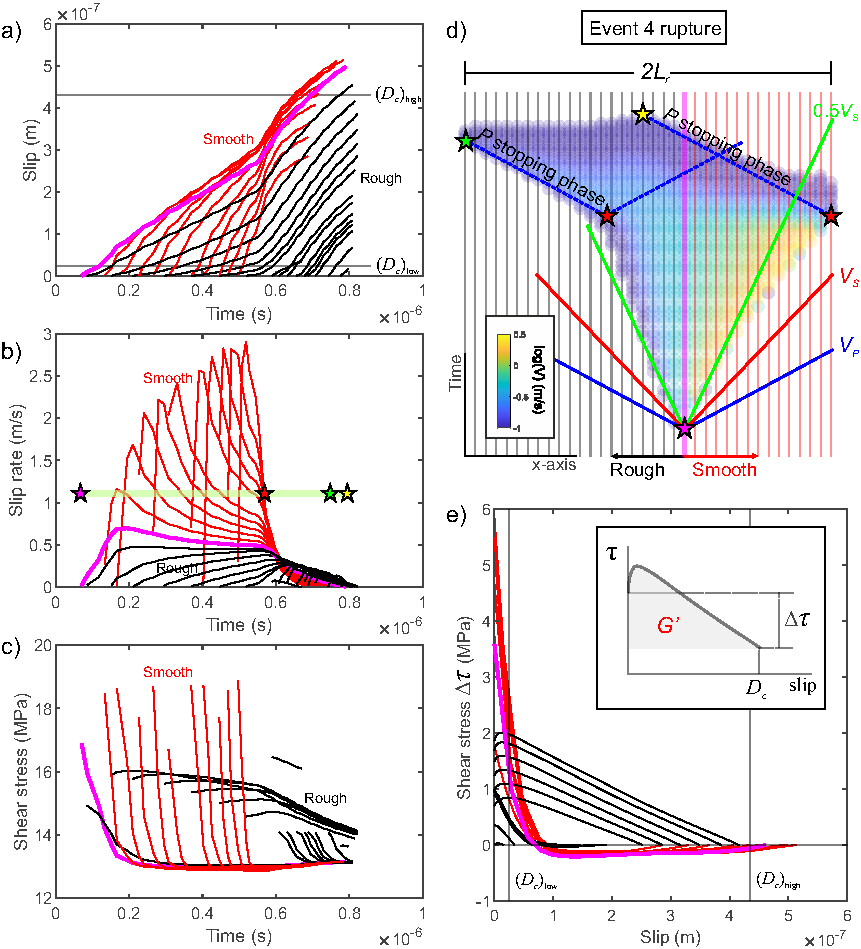
\includegraphics{FIG9.pdf} 
	\caption{Rupture complexity of Event 4 in Figure \ref{fig8}(d) and (e) in space-time plots.  \textbf{(a)} Temporal evolution of slip along 25 different transects of the rupture spaced evenly on the fault. \textbf{(b)} Temporal evolution of slip rate along the same transects as in (a). Key moments of the rupture are given by the colored stars. \textbf{(c)} Temporal evolution of shear stress for the same positions as in (a). \textbf{(d)} Space-time plot of the rupture with the transects depicted graphically. \textbf{(e)} We investigate the traction-slip from each transect. The inset image shows how we measure (static) stress drop ($\Delta \sigma$) and effective fracture energy ($G^{'}$) for each position on the fault.}
	\label{fig9}
	
\end{figure}

These plots provide a more concise temporal understanding that clearly shows the diversity in the temporal evolution of: (a) slip, (b) slip-rate and (c) shear stress along the transects shown in Figure \ref{fig9}(d). In Figure \ref{fig9}(a) we observe that the rupture has a non-uniform distribution of accumulated slip. The average slip along the 25 estimates was $\delta$ = 0.37 $\mu$m.  This average can be used with the relationship for seismic moment $M_{0}$ given by \citeA{Aki1966}: 

\begin{equation}
M_{0} = G A \delta, 
\label{eq9}
\end{equation}

\noindent where $A$ is the fault area and $\delta$ is slip. For a penny-shaped fault $A$ = $\pi r^{2}$ and for a square fault $A$ =$(2L_{r})^{2}$.  We calculated the average slip from the final amount on each transect of the fault which was $\delta$ = 0.37 $\mu$m for this example.  Using this formula we find this rupture to have an average scalar seismic moment $M_{0}$ = 0.0014 N$\cdot$m. This is equivalent to a moment magnitude $M_{w} = (2/3)\cdot(log_{10}(M_{0})-9.05) = -7.94$ \cite{Kanamori1975}.  

In Figure \ref{fig9}(b), we see the complexity in slip rate along each transect of the rupture more clearly. For further clarity, the important aspects of the rupture (colored stars) are superimposed and correspond to the important moment associated with Event 4 rupture (stars). As mentioned earlier, the rupture appears to have higher slip rates along the smoother section of the fault, whereas the rough section shows more resistance to the rupture.  This is seen in Figure \ref{fig9}(c) in that the smooth portions of the fault (red transecting lines) drop shear stress very quickly with little accumulated slip, whereas the rough sections (black transecting lines) offer resistance and exhibit slower rates of weakening.

We use this analysis to better understand the intrinsic source properties of the rupture and how it varied along the fault. In Figure \ref{fig9}(e) we show the normalized slip-traction relationship for each transect of Figure \ref{fig9}(a). The normalization is with regards to the inset image that describes how to calculate stress drop ($\Delta\tau$) and effective fracture energy ($G^{'}$), also known as breakdown work in the literature \cite<e.g.>[]{Tinti2005, Cocco2016}. We see from Figure \ref{fig9} that there appears to be obvious participation of both the rough and smooth sections of the fault. For clarity we have highlighted the critical slip weakening distance for both the smooth $(D_{c})_{low}$ and rough section of the fault $(D_{c})_{high}$. We see that in some cases slip was greater than $(D_{c})_{high}$ which can be explained as dynamic overshoot \cite{Madariaga1976}. Calculating $\Delta \tau$ is relatively straight forward, but to determine the effective fracture energy $G^{'}$, we numerically integrated the area under this curve. For Event 4, the average stress drop was $\Delta\tau$ = 3.25 MPa and average effective fracture energy $G^{'}$ = 0.13 J/m$^{2}$.

%%%%%%%%%%%%%%%%%%%%%%%%%%%%%%%%%%%%%%%%%%%%%%%%%%%%%%%%%%%%%%%%%%%%%%%%%%%%%%%%%%%%%%%%%%%%%%%%%%%%%%%%%%%%%%%%%%%%%%%%%%%%%
%\subsubsection{Non-uniform characteristic length scale $L_{b}$}

%Many RSF studies model frictional behavior using a combination of VS and VW regions to produce the complex frictional behavior. These studies benefit in that the description of the critical length scale $L_{b}$ (equation \eqref{eq8b}) is constant within a given region.  However, these models may be susceptible to the peescription of the geometries of the VS to VW regions, which we try to avoid with our cutting plane method.  

%As we see from Figure \ref{fig9}, our ruptures are quite complex. We see that along the down-strike propagating rupture front has bridged a few smooth sections of the fault before arresting (green star).  The heterogeneity in $D_{c}$ will cause the $L_{b}$ vary at each point on the fault.

%\begin{figure}
%	\centering
%	\includegraphics{FIG9a.pdf} 
%	\caption{Relationship between the average cohesive length scale $\bar{L}_{b}$ to: \textbf(a) the average critical slip weakening distance $D_{c}$ along a rupture and \texbf{(b)} the length of the rupture $L_{r}$. \textbf(c) Evolution of $\left<D_{c}(t)\right>$ with duration of rupture for all events in the O17.5 $D_{c}$-model.}
%	\label{fig9a}
%\end{figure}

%Figure \ref{fig9a}(a) shows the variation in $\bar{L}_{b}$ for each rupture recorded. This was calculated from averaging $\left<D_{c}\right>$ on each transect of the rupture in Figure \ref{fig9}.  We have normalized the average $\left<D_{c}\right>$ by $(D_{c})_{low}$ and we see that the average falls within the upper and lower bounds prescribed by each model. We see that $\bar{L}_{b}$ varies linearly, as expected from the inset equation, but the distribution and range is related to the spatial variations in $D_{c}$ along the rupture. In Figure \ref{fig9a}(b) we show the relationship between rupture length $L_{r}$ and $\bar{L}_{b}$.  We see that there is no clear correlation between length of $L_{r}$ and $\bar{L}_{b}$. However, we do see that $\bar{L}_{b} > L_{r}$, which is not a common observation for RSF studies \cite{Chen2009, Cattania2019}. The just mentioned studies showed only aseismic behavior when $\bar{L}_{b} > L_{r}$. In our case, initiation of the rupture on the smooth sections caused $\bar{L}_{b}$ to fluctuate and increase with time.  This may be indicative of an arrest mechanism for the heterogeneous $D_{c}$-model.

%In Figure \ref{fig9a}(c) we show how the average critical slip weakening distance varies with rupture time $\left<D_{c}(t)\right>$. To do so, we use the cumulative mean of $D_{c}$ on rupturing elements as the rupture evolves.  We show the results for the O17.5 model here and show that ruptures must all depart from either $(D_{c})_{low}$ (blue) or $(D_{c})_{high}$ (red).  As expected, the ruptures tend to converge to a value between these bounds but no clear value of $\left<D_{c}\right>$ is observed for this model. This non-uniqueness differs between ruptures due to the complexity in stress state that evolves continuously throughout the simulations. According to equation \eqref{eq8b}, as $\left<D_{c}(t)\right>$ evolves over rupture time, the instantaneous average $\bar{L}_{b}$ will vary with the expanding rupture.  This helps to explain why $\bar{L}_{b}/L_{r} > 1$ for many of the ruptures shown in Figure \ref{fig9a}(b).

\subsubsection{Seismic moment versus source size}

We investigate seismic source properties and their scaling relationships over multiple ruptures and by using different models. In Figure \ref{fig10}(a) we examine the relationship between source area $A_{r} = (2\cdot L_{r})^{2}$ and seismic moment $M_{0}$. Source properties in this study are determined using dynamic RS models but this model is simplified in our analysis to the quasi-dynamic case. Due to the simplification, our model does not produce seismic waves \cite{Freund1990, Rosakis2002}. However, we know these waves were produced since they were recorded using the array PZT sensors. Estimations of source properties inferred from seismic waves are already available in the concerted study by \citeA{Selvadurai2019}.  Kinematic source shear crack models \cite{Brune1970, Madariaga1976, Hanks1979} are commonly used to interpret source information of moderate to small to medium earthquakes where finite source inversion is not possible. Please see table 2 in \citeA{Cocco2016} for an overview of studies that employ these techniques for a range of earthquakes sizes and settings. We use the RSF results from this study to compare the kinematic estimates of source properties to those made independently here using roughness-based dynamic friction models. \citeA{Chen2009} have prepared a similar plot, comparing source properties from RSF model to seismologic estimates; however, to the authors' knowledge this has not been directly shown in a laboratory setting at such detail and more control on features affecting kinematic source models, such as wave scattering in heterogeneous media, which is not the case for PMMA.

In Figure \ref{fig10}(a) we show the results five $D_{c}$-models (circles) against the kinematic estimates made from P and S wave arrivals (triangles) using shear crack models detailed by \citeA{Selvadurai2019}. The kinematic estimates shown here used assumptions that the instantaneous rupture velocity was $V_{r} = 0.9 \cdot V_{S}$ following the numerical simulations by \citeA{Madariaga1976}. We see that the RSF models produce similar estimates of source length scale and seismic moment from the kinematic source models.  The general scaling relationship $M_{0}\propto$ (length scale)$^{3}$ is observed for both methods to calculate source properties.

\subsubsection{Frequency-magnitude distribution}

We look at the frequency-magnitude distributions (FMDs) from the acoustic emission (AE) data and RSF model in Figure \ref{fig10}(b). The colors are the same as legends in Figure \ref{fig10}(a).  The Gutenberg-Richter \cite{Gutenberg1944} relationship is the most commonly observed empirical relationship in seismology.  It states that large earthquakes occur less frequently than small earthquakes following the standard relationship $log_{10}(N)= a_{GR} - b_{GR}M$, where $N$ is the number of events equal or above magnitude $M$ and $a_{GR}$ and $b_{GR}$ are constants \cite<e.g.>[]{Wiemer2002}.  This relationship is commonly used to convey hazard and risk by detailing the productivity ($a_{GR}$-value) and size distribution ($b_{GR}$-value) in the volume of interest.  While these values are typically used to assess volumes of rock, we employ it here to study patterns in on-fault seismicity -- caution should be used if extrapolating any findings to natural faults where off-fault seismicity might factor into the observations.  

Figure \ref{fig10}(b) shows the different seismic responses and a $b_{GR}$ = 1 is shown for reference. We note that the $D_{c}$-models O10 (red) and O20 (blue) do no appear to capture the full catalog of AE estimates for P waves (thick orange line) or S waves (thick gray line).  The O15 (green) show a relatively similar productivity $a_{GR}$ but slightly lower $b_{GR}$-value. Both O17.5 and O18.5 (gray) show the highest level of productivity.  We mainly use the FMD metrics as qualitative comparison of the two different source modeling methods. \citeA{Goebel2016} also investigated the effect of roughness on b-values and found that polished faults had lower b-values than roughened samples. This appears to follow our results if we consider that `smoother' is related to smaller levels of heterogeneity (O10, red) has the lowest b-value and it progressively increases until the relatively `rougher' O18.5 model. However, the b-value drops again for the O20-model, which coincides with a more creep dominated  frictional response (Section \ref{Recurrence times}) but we are not sure how to interpret this.

\begin{figure}
	\centering
	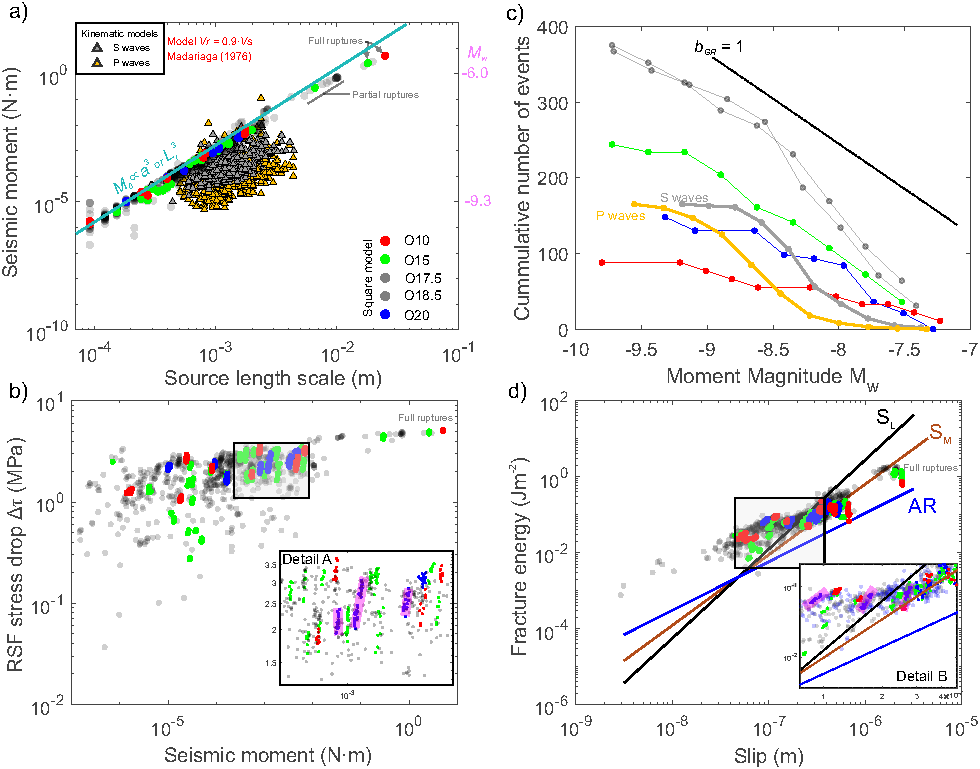
\includegraphics[scale = 0.95]{FIG10.pdf} 
	\caption{\textbf{(a)} Source length scale is calculated from the numerical models with various levels of heterogeneity (colored circles) and compared to their respective scalar seismic moment $M_{0}$. These are compared to the kinematic estimate of source properties determined using shear crack models described in \citeA{Selvadurai2019} for both P and S waves (triangles). \textbf{(b)} Frequency-magnitude distributions (FMDs) are given for each catalog shown in (a).  Values for FMD properties $a$ and $b$ are given in the text, and the magnitude of completeness $M_{c}$ is shown as color coded arrows. \textbf{(c)} Relationship between frictional stress drop ($\tau_{d}$) and rupture area. \textbf{(d)} Effective fracture energy ($G^{'}$) versus slip is shown. We compare the models to empirical scaling estimates from laboratory seismicity \cite<black line>{Selvadurai2019}, mining seimsicity \cite<brown line>{Selvadurai2019} and field estimates \cite<blue line>{Abercrombie2005}, in which the latter has been extrapolated.}
	\label{fig10}
\end{figure}

\subsubsection{RSF Stress drop with seismic moment}

Figure \ref{fig10}(c) looks at the relationship between stress drop and seismic moment release given by equation \eqref{eq9}. We see that event with lower $M_{o}$ appear to have slightly diminished levels of stress drop $\Delta \tau$. We found this was not to be a feature of under-sampling and is was related to the amount of stress corrosion that will occur on smaller asperities as portions of their shear stress is partially released in the nucleation phase prior to them transitioning to a becoming a dynamic event. This is discussed in more detail in Section \ref{RSFvEshelby}. Detail A shows enhanced view of only the O10, O15 and O20 models, where we noticed variable stress drops earthquakes that had very similar magnitude, a feature to repeating earthquakes observed recently by \citeA{Cauchie2020} when revisiting seismicity patterns from the 1993 stimulation of a geothermal reservoir in Soultz-sous-For\^{e}ts, France.

\subsubsection{Fracture energy scaling}

We look into the scaling behavior between effective fracture energy and slip and the effect of the heterogeneous $D_{c}$. \citeA{Abercrombie2005} showed that effective fracture energy $G^{'}$ scales with slip ($\delta$) according to the empirical relationship $G^{'} \propto \delta^{\gamma}$. This is of interest to the seismologic community since it helps to understand how strain energy is partitioned during rupture. Whether this scaling relationship holds universally is not agreed upon. Laboratory experiments where $G^{'}$ is directly measured show that a variety of mechanisms might lend to deviation from the trend documented by AR.  For example, frictional mechanisms such as flash-heating of asperities caused by elevated temperatures on the fault from frictional dissipation \cite<e.g.>[]{Passelegue2016, Brantut2017} or off-fault damage due to high strain rates in the vicinity of rupture tip \cite<e.g.>[]{Andrews2005, Nielsen2016}, among other mechanisms, can lead to deviations from the AR scaling trend. \citeA{Selvadurai2019} put together a compendium of seismologic estimates from natural, mining and laboratory studies. He found that the empirical trends vary at each scale.

In Figure \ref{fig10}(d) we compare the estimates of $G^{'}$ for the different models using the methods described in Section \ref{Constitutive}. These are compared to the previously discussed empirical relationship for shear crack source models from laboratory ($S_{L}$, $\gamma = $2.35) and mining estimates ($S_{M}$, $\gamma = $1.86) \cite{Selvadurai2019}. We also compared this to get estimates made at regional scales from natural earthquakes (AR, $\gamma = $1.28) following the observations by \citeA{Abercrombie2005}.  This empirical relationship was later confirmed by \citeA{Mai2006}.  We see that the results from the model tend to follow the same slope as AR but if we look more closely, shown in Detail B, we see that some of the repeating patches show steeper trends in scaling (see highlighted clusters). This can be explained by the fact that there were preferential patches -- worn smooth sections -- that, when they ruptured, would remain relatively constant in size but the stress drop varied as is shown in Detail A in Figure \ref{fig10}(b). This behavior have been seen in reservoir-scale studies in a recent seismological study by \citeA{Cauchie2020} and might describe why repeaters are observed on worn and mature faults in nature (see discussion in Section \ref{Repeaters}). 

\subsubsection{Recurrence rates}
\label{Recurrence times}
In Figure \ref{fig11}(a) we show the average slip (black) and shear stress (red) for a small portion of simulations for stong barriers O20 (left-hand side, LHS) to weaker barriers O10 (right-hand side, RHS). The transitional case O17.5 is shown in the middle.  We see the average behavior of the fault transition from one that is creep-dominated (O20) to one that stick-slip dominated (O10).  For this analysis, we look closely at the recurrence rate $T_{r}$ of the localized events.  We consider $T_{r}$ to be the time between any two events at any location on the fault.  Since we do not consider nucleation processes in this analysis, we look at the recurrence time between two sequential ruptures. To disseminate triggered seismicity versus repeater events, we adopt the methodology described in \citeA{Lengline2009}. They looked at the frequency distribution of the recurrence times normalized by the average recurrence time $T^{*}_{r}$.  They found that below $T_{r}/T^{*}_{r} <$ 0.1 the distributions followed a power-law distribution, which is consistent with Omori's law that described aftershocks in nature \cite<e.g.>[]{Lengline2009}. 

In Figure \ref{fig11}(b) we show the probability distribution of $T_{r}/T^{*}_{r}$ for the five $D_{c}$-models. The purple region highlights portions of the distribution that are likely not triggered events. A small fall-off is observed when $T_{r}/T^{*}_{r} <$ 1e-6 and is likely due to saving computational solutions every 10 times steps because of memory constraints, thus decreasing information for those bins. We see that for the creep-dominated O20 model there is relatively equal probability in recurrence time but a slight increase in  $T_{r}/T^{*}_{r} >$ 0.1 lending to the idea that this is a more repeater-like behavior. In the transitional models (O18.5, O17.5 and O15) we fit a power law distribution (gray lines) between 1e-5 $< T_{r}/T^{*}_{r} <$ 0.1 and found its slope to decrease as the heterogeneity was decreased. We note a small `bump' in probability above $T_{r}/T^{*}_{r} >$ 0.1, denoted with the small arrow in O15. This appears to have been amplified in O10, or the stick-slip dominated model, and this is discussed later in the context of possible ties of foreshock-like behavior.

\begin{figure}
    	\centering
	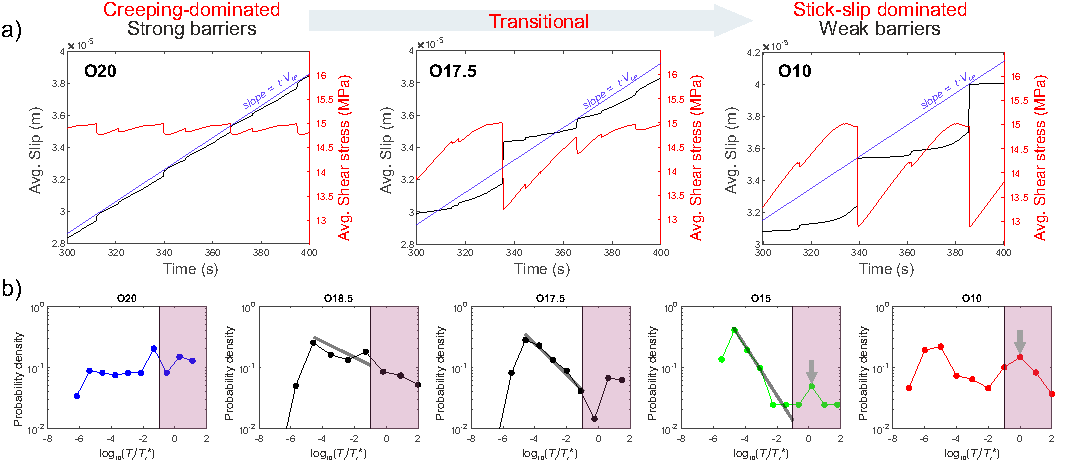
\includegraphics[scale = 0.9]{FIG11.pdf} 
	\caption{Earthquake recurrence rate for each $D_{c}$-model from higher O20 to lower O10 levels of strength heterogeneity. (\textbf{a}) We show the average behavior of the entire fault for small portion of time $t$ 300 to 400 s for the O20 (creeping-dominated), O17.5 (transitional) and O10 (stick-slip dominated) models. (\textbf{b}) Probability density of the lognormal distribution of normalized recurrence rates $T_{r}/T^{*}_{r}$ for all models. The probabilities above $T_{r}/T^{*}_{r} >$ 0.1 in purple are highlighted.}
	\label{fig11}
\end{figure}

%%%%%%%%%%%%%%%%%%%%%%%%%%%%%%%%%%%%%%%%%%%%%%%%%%%%%%%%%%%%%%%%%%%%%%%%%%%%%%%%%%%%%%%%%%%%%%%%%%%%%%%%%%%%%%%%%%%%%%%%%%%%%
\subsection{\textit{Composite}-model}
So far we have chosen to investigate the $D_{c}$-model. We note that this study aims at providing an understanding of the differences between RSF- and AE-driven estimates of source properties. We are not attempting to exactly match each independent measurement to each other since we believe that both methods have considerable assumptions; furthermore, perfect matching by tweaking input parameters defeats the inherent benefit of these comparison exercises.

For completeness we investigate the \textit{Composite}-model that aims at capturing additional complexity that may exist in the spatial distribution in normal stress. We see from the experimental observations with the pressure sensitive model (Figure \ref{fig4}(b)) that normal stress asperities exist. According to the contact mechanics literature \cite{Nayak1971, Nayak1973}, the preferentially smooth sections above the cutting plane (Figure \ref{fig3}) will likely produce localized patches of normal stress asperities. To model such conditions, we again use the scaling function. However, now on smooth sections (low $D_{c}$) we prescribe constant normal stress $\sigma_{high}$ = 25 MPa.  In rough sections, we apply a constant low normal stress level, which was set to the lower measurable limit of the pressure sensitive film $\sigma_{low}$ = 12 MPa \cite{Selvadurai2015a}. 

In Figure \ref{fig12}(a) we show a section of the spatial heterogeneity from $x$ =  5 to 8 mm for variations in $\sigma$ (red) and $D_{c}$ (blue).  The scaling function was chosen to be O20, which was a model that had a relatively well-behaved response from before.  We use the same methods to calculate source properties and examine similar relationships for this composite-model (O20C).

\begin{figure}
	\centering
	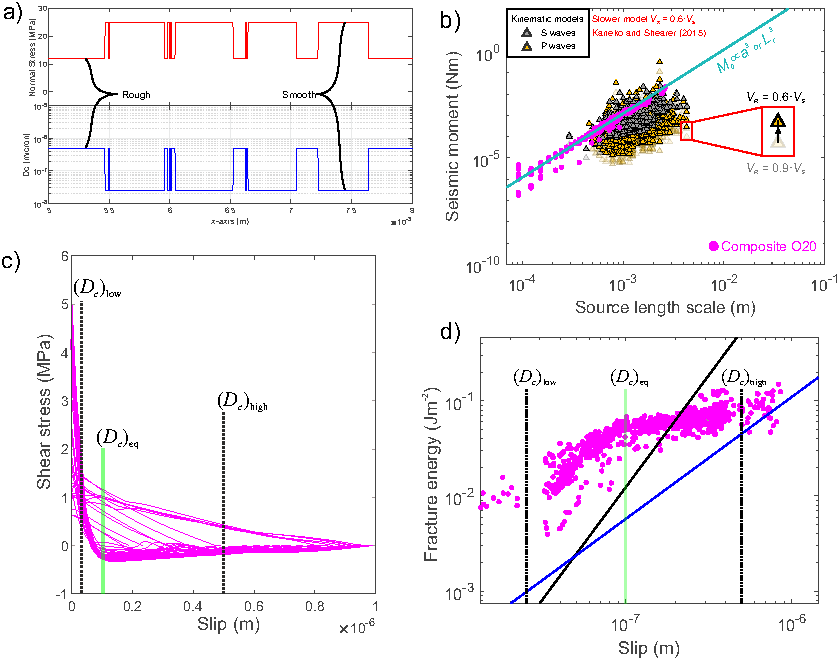
\includegraphics{FIG12.pdf} 
	\caption{Results from the \textit{Composite}-model. \textbf{(a)} A small section of the 1D fault form $x$ = 5 to 8 mm showing the spatial variation in both $D_{c}$ and $\sigma$. \textbf{(b)} The scaling relationship between $A_{r}$ and $M_{0}$ (gray circles) is compared to the corrected kinematic estimates of source properties from \citeA{Selvadurai2019} (triangles).   \textbf{(c)} Constitutive behavior for a large event in the \textit{Composite}-model. \textbf{(d)} Relationship between effective fracture energy $G'$ and slip $\delta$. Empirical relationship between black and blue lines is similar to the one shown Figure \ref{fig10}(d).}
	\label{fig12}
\end{figure}

Figure \ref{fig12}(b) shows the relationship between $M_{0}$ and $A_{r}$. We find that it produces similar estimates to the kinematic shear crack model shown in Figure \ref{fig10}(a). However, here we have made an additional improvement assumptions in the shear crack model regarding the rupture speed.  We now apply a correction factor to account for slower ruptures in the kinematic models for example $V_{r} = 0.6\cdot V_{S}$.  This analysis was performed by \citeA{Kaneko2015} for a range of rupture scenarios: circular or elliptical and symmetric or asymmetric.  They found that decreasing the rupture speed can produce deviations of up to 2.5 times more stress drop depending on the model and the wave.  From the RSF simulations, an example shown in Figure \ref{fig9}(d), we found that the average rupture velocities were much lower than the 0.9$\cdot V_{S}$, more close on average to 0.6$\cdot V_{S}$.  From table 1. in \citeA{Kaneko2015}, we updated the estimates form \citeA{Selvadurai2019}, which minimized the deviations between the kinematic (triangles) and RSF (circles) estimates of source properties.  The correction factor used to scale the original kinematic estimates were taken from asymmetric circular asperity model for a rupture velocity $0.6\cdot V_{S}$ that led to an increase in seismic moment of 2.63 and 2.74 from P and S waves estimates, respectively.

Figure \ref{fig12}(c) shows the constitutive shear stress versus slip behaviour for a large random asperity. For reference, we mark the levels of $(D_{c})_{low}$, $(D_{c})_{eq}$ and $(D_{c})_{high}$.  The term $(D_{c})_{eq}$, or equivalent critical slip weakening distance, appears to be a representative critical slip weakening distance that always lies between the two $D_{c}$ limits but will likely vary on each rupture and is a function of the ratio of high to low resistance of the interface participating in rupture.  

Using the methods described in Figure \ref{fig9}, we looked at the relationship between $G^{'}$ and slip. In Figure \ref{fig12}(d) we see that the relationship appears to have a ``kink''.  This kink is observed about $(D_{c})_{eq}$. As the smooth rupture front moves out, it propagates more efficiently into the smooth section but still accrues large amounts of fracture energy per unit slip as it moves less quickly into the rough-barrier in the opposite direction. As the efficient rupture encounters its first barrier, it is either arrested or breaks through. This might indicate that the equivalent critical slip weakening distance $(D_{c})_{eq}$ could be related to the average length scale of worn sections and the level of the discontinuity it encounters.  



%%%%%%%%%%%%%%%%%%%%%%%%%%%%%%%%%%%%%%%%%%%%%%%%%%%%%%%%%%%%%%%%%%%%%%%%%%%%%%%%%%%%%%%%%%%%%%%%%%%%%%%%%%%%%%%%%%%%%%%%%%%%%
\section{Discussion}
We have summarized findings from a well-documented laboratory experiment where worn surfaces of two PMMA blocks were pressed together, forming a frictional interface, then sheared to failure \cite{Selvadurai2015, Selvadurai2015a, Selvadurai2017}. Macroscopically, the fault displayed a quasi-statically slipping nucleation zone that expanded until reaching a critical size, upon which the entire fault produced macroscopic stick-slip events (see Figure \ref{fig1}(b)).  Slow slip was captured using an array of low-frequency sensors (Figure \ref{fig1}(c)). As slow slip accumulated, high frequency impulsive emissions were also detected using acoustic emission sensors (Figure \ref{fig1}(d)).  These were in fact elastodynamic stress waves (Figure \ref{fig1}(e)) that contain source information associated with small seismic asperities that persisted in a larger slow sliding region.  

Upon inspection, the fault appeared to be worn in the region of the fault that produced seismicity. Roughness measurements were taken (Figure \ref{fig2}) and were used to impose heterogeneity in a quasi-dynamic RSF model. Roughness profiles appeared to show preferential wear (smooth flat asperities) that is commonly mentioned in the tribological literature. A cutting plane method (Figure \ref{fig3}), was used to mathematically quantify the spatial variation in smooth and rough sections. Two sets of RSF properties were chosen based on the fact that smooth surfaces have lower critical slip weakening distance $D_{c}$ than rougher sections.  

The models showed very complex behaviour (Figure \ref{fig7}) that differed from the homogeneous case (Figure \ref{fig5}).  We developed algorithms to isolate ruptures (Figures \ref{fig8} and \ref{fig9}).  These allowed us to estimate a range of source properties, such as scalar seismic moment ($M_{0}$), rupture length ($L_{r}$), seismic slip ($\delta$), RSF stress drop ($\Delta\tau$), RSF fracture energy ($G'$), frequency-magnitude distributions and recurrence rates of five different $D_{c}$-models and a composite-model (Figures \ref{fig10}, \ref{fig11} and \ref{fig12}). These calculations were compared to independently estimated source properties made from interpreting the seismic waves \cite{Selvadurai2019}.  Building from our assumption that spatial variations in roughness caused similar variations in $D_{c}$, we found that estimates of source size and moment release were similar in both methods; however, some discrepancies exist. 

%%%%%%%%%%%%%%%%%%%%%%%%%%%%%%%%%%%%%%%%%%%%%%%%%%%%%%%%%%%%%%%%%%%%%%%%%%%%%%%%%%%%%%%%%%%%%%%%%%%%%%%%%%%%%%%%%%%%%%%%%%%%%
\subsection{Dynamic RSF versus kinematic estimates of source features}
Our model has successfully reproduced aspects of seismicity that were produced from an experimental fault using two independent methods.  It appears as if this is the first time such a highly comparative study has been performed and, more so, a RSF fault that has used experimental measurements to make a pseudo-roughness model. Our model does not just take information from the roughness scans (Figures \ref{fig2} and \ref{fig3}) but also builds on the novel estimates of asperity normal stress using a pressure sensitive film to better constrain the mesoscopic section of fault that is responsible for concomitant slow and fast sliding (Figure \ref{fig4}). 

The model displays a wide variety of complexity at the mesoscopically (Figure \ref{fig7}) and microscopically (Figures \ref{fig8} and \ref{fig9}). Ruptures showed similar scaling behavior between seismic moment and source radius as was found by analyzing ground vibrations produced by the seismic waves (see Figure \ref{fig10}(a)). While the dynamic and kinematic source estimates highlighted here differ slightly, the magnitude and trends between estimates are similar and, without any \textit{a priori} knowledge, comparing these two different models is an important step forward.  Discrepancies may be caused by numerous features that we discuss next, but similar types of laboratory study, with more controlled and well-posited experiments, may help quantify how influential these assumptions affect our shear crack kinematic model.

Our numerical model was only quasi-dynamic and fully dynamic solvers may be needed.  Our numerical model does not incorporate dilation \cite{Selvadurai2018}, which, even in a static sense might affect behavior and stress intensity factors. The 1-D approximation might not capture some of the inherent 2D spatial complexity in the preferentially worn surface.  This will be subject of future work. There are numerous simplifications in the kinematic approach that may also impose errors in estimates of source properties. These are well covered by \citeA{Selvadurai2019}. While we attempted our best to absolutely quantify their instruments response with high-frequency sources (see fig. 2 therein), frequency dependent attenuation of PMMA might not have been characterized sufficiently with their empirical Green's functions. The main author is currently investigating numerical calibration methods to quantify this more accurately moving forward \cite{Wu2020}.

We see that stress drop is dependent on the rupture velocity ($V_{r}$) \cite{Kaneko2015}. From our RSF models we needed to correct the simple circular asperity model used by \citeA{Selvadurai2019}, for a slower rupture velocity ($V_{r} = 0.6\cdot V_{S}$).  In most cases, shear crack models assume rupture velocities of 0.9 or 1.0$\cdot V_{S}$ and there is yet to be a justifiable reasoning as to why this is assumed \cite{Cocco2016, Selvadurai2019}. We found that results from the RSF modelling, rupture velocities are more likely closer to 0.6$\cdot V_{S}$ making this analysis a useful one to better constrain parameters such as rupture velocity. From the improved understanding, we were able to apply numerical studies performed by \citeA{Kaneko2015} to update the kinematic source estimates made for faster rupture velocities.  This correction minimized the deviations between source estimates from the independent models. This type of analysis could help to better understand the effects of asperities and barriers on the choices of parameters in kinematic source models, using a laboratory-based understanding, that can better constrain assumption when interpreting small to moderate natural earthquakes.

\subsection{Comparison of RSF stress drop versus shear crack stress drop}
\label{RSFvEshelby}
The theory surrounding a penny-shaped shear crack embedded in an elastic homogeneous material is frequently employed to estimate the stress drop from an earthquake following the derivation by \citeA{Eshelby1957}. This theory is used to calculate stress drop ($\Delta\sigma$), which is different than the RSF stress drop $\Delta\tau$ in terms of the defining frictional laws. Stress drop calculated on a shear crack is the average shear traction required to dislocate the interface by the amount of average slip $\delta$ in equation \eqref{eq9}. For a circular shear crack embedded in a Poissonian material with radius $r$, stress drop $\Delta\sigma$ is given as: 

\begin{equation}
\text{Circular}: \Delta\sigma = \left(\frac{7\pi}{16}\right) \frac{G \delta}{r}.  
\label{eq10}
\end{equation}

\noindent For a rectangular fault with side lengths $L$ x $W$ we can rewrite this stress drop as \cite<Appendix A,>[]{Kato2003}:

\begin{equation}
 \text{Rectangle}: \Delta\sigma =  \frac{2G\delta}{3\pi} \left(\frac{3L^{2} + 4W^{2}}{LW\sqrt{L^{2} + W^{2}}}\right),   
\label{eq10a}
\end{equation}

\noindent and for the square crack ($L=W$) with side length $2L_{r}$ this simplifies to:

\begin{equation}
 \text{Square}: \Delta\sigma = \left(\frac{7\sqrt{2}}{3\pi}\right)\frac{G\delta}{L_{r}}.   
\label{eq11}
\end{equation}

\noindent Estimating stress drop by using this method remains controversial in the seismological community \cite{Beresnev2001}. Assumptions regarding equations \eqref{eq10} to \eqref{eq11} might not accurately capture the physical realities of the problem. For example, there is no frictional dissipation (heating) and the process of dislocating the interface in shear is solved in an entirely reversible manner; if we were to unload the static shear traction $\Delta\sigma$, the crack would return to its original position, which appears to be ill-conceived from at minimum the visual evidence of damage on and near faults in nature \cite<e.g.>[]{Mitchell2009}. While there are inherent assumptions embedded in the phenomenological RSF formulation, it is aimed to provide a more representative approximate behavior of the physical processes and to better capture sources of energy dissipation not present in a model with reversible assumptions.

\citeA{Cattania2019} have performed an important study on this topic. They compared rupture behavior of a circular VW weakening asperity with radius $r$, surrounded by a creeping VS region, using a quasi-dynamic RSF analysis \cite<see also>[]{Kato2003, Chen2009}. They found that aseismic preparation of the patch affected the level of seismically released stress drop. In this study we do not quantify aspects of nucleation explicitly but we find similar trends existed in our estimates of seismic RSF stress drop $\Delta\tau$ when compared to the shear crack stress drop $\Delta\sigma$ from equation \eqref{eq11}.

To compare the two models, we first look at the computed RSF stress drop $\Delta\tau$ for the isolated events in the $D_{c}$- and composite-models. From these events we also have the metrics for slip $\delta$ and rupture length half-length $L_{r}$. Metrics of $\delta$ and $L_{r}$ are used with equation \eqref{eq11} to estimate the shear crack stress drop $\Delta\sigma$. By normalizing the RSF estimates of stress drop $\Delta\tau$ by $\Delta\sigma$ we find that stress drop on smaller ruptures is consistently overestimated by the stress drop from the crack model and that this overestimate decrease weakly with $L_{r}$ (Figure \ref{fig13}(a)). \citeA{Cattania2019} show similar results and concluded that this is due to portions of shear stress being pre-released in the nucleation phase, what we call stress-corrosion. We believe that this is the case for our RSF models.  This is verified by re-analysing the ruptures but artificially setting the threshold for seismicity two orders of magnitude lower $V_{dyn}$ = 0.001.  We find that the differences between $\Delta\tau/\Delta\sigma$ are less on the smaller ruptures since the shear stress corrosion associated with the nucleation phase is now captured.

\begin{figure}
       	\centering
	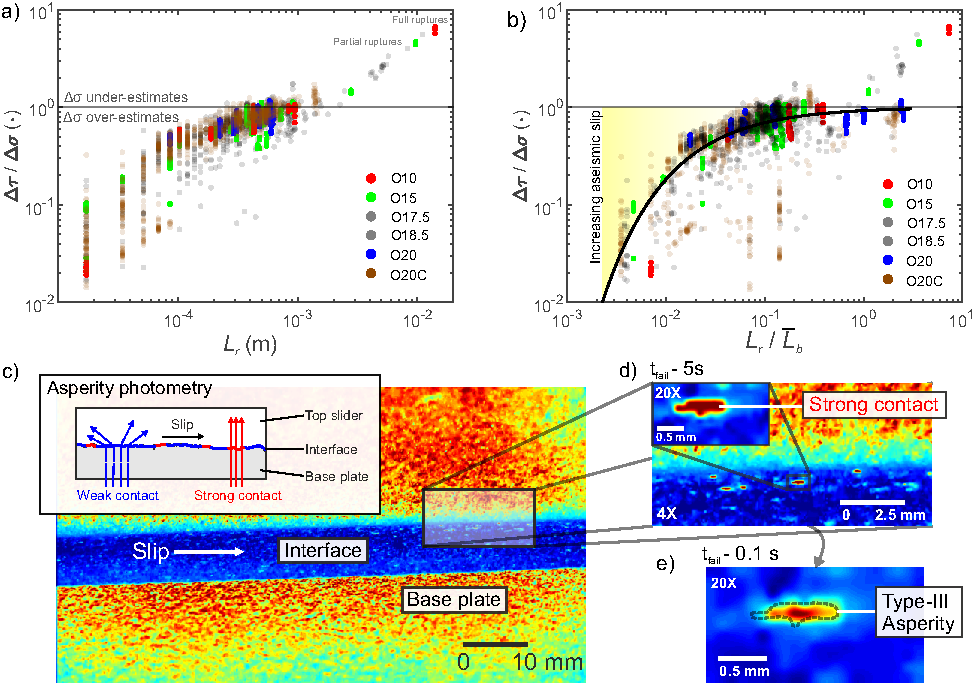
\includegraphics[scale= 0.95]{FIG13.pdf} 
	\caption{\textbf{(a)} Comparison of RSF stress drop ($\Delta\tau$) and the shear crack stress drop ($\Delta\sigma$, equation \eqref{eq11}) with side length $L_{r}$.  \textbf{(b)} The ratio of $\Delta\tau/\Delta\sigma$ is compared to the normalized side length $L_{r}/\bar{L}_{b}$. The yellow region shows the range of asperities that will have a portion of their shear stress alleviated in the nucleation phase (stress corrosion). \textbf{(c)} [Adapted from \citeA{Selvadurai2015}] Photometry was performed through the transparent side of the PMMA top slider block. A schematic diagram shows how strong contacts (red) will transmit light whereas weak contacts will diffract light (blue). This is superimposed over a sample image of the interface (blue) used to qualitatively study the strong contacts. The image color is from blue to red which translated dark to light in physical terms. This image was taken exactly 5 seconds before macroscopic stick-slip failure. \textbf{(d)} Enhanced (4X) view of the interface where strong contacts (red pixels) were present. A single large strong contact is enhanced (20X) for the frame taken at $t_{fail}$-5 seconds.  \textbf{(e)} Changes in light transmitted through the large contact changed over the $\sim$ 4.9 seconds of the macroscopic nucleation phase, which might be qualitative evidence of stress corrosion. The periphery of the strong contact pixels in (d) is shown (dashed-line) for comparison.}
	\label{fig13} 
\end{figure}

Theoretical studies in the behavior of RSF models have been used to non-dimensionalize the problem and identify parameters such as $L_{c}$ (equation \eqref{eq8}) and $L_{b}$ (equation \eqref{eq8b}) \cite{Ruina1983, Ranjith1999, Rubin2005, Ampuero2008}. \citeA{Cattania2019} applied this theory to understand how the circular asperity behaves with respect to the ratio of $L_{r}/L_{b}$. In Figure \ref{fig13}(b), we estimate $\bar{L}_{b}$ but this is clearly different from standard description of $L_{b}$ given in equation \eqref{eq8b} since $D_{c}$ varies with $x$.  We estimate $\bar{L}_{b}$ using the average $D_{c}$ with elements that participated in the rupture.

but show clearly complex behavior due to the prescription of $D_{c}$ in the model.  The trend shown in Figure \ref{fig13}(b) shows that smaller values of $L_{r}/\bar{L}_{b}$ over-predicted stress drop when using the shear crack model $\Delta\sigma$ since this model does not account for `stress corrosion' in the nucleation phase.

The trends shown in our models are predicted theoretically by \citeA{Cattania2019} (see fig. 13 and appendix C therein).  They summarized the behavior of a single circular asperity with radius $r$ into four types of behaviors \textbf{Type-I}: fully aseismic asperity; \textbf{Type-II}: surrounding creep erodes asperity and rupture nucleates from the center but stress drop increases weakly with $r$; \textbf{Type-III}: surrounding creep partially erodes asperity and rupture nucleates with stress drop strongly linked to $r$; \textbf{Type-IV}: minimal stress corrosion and energy required to propagate a rupture is less than that needed to nucleate resulting in a partial rupture. In our study it is difficult to absolutely pin down the true value of $L_{c}$ and $L_{b}$ due to the model heterogeneity, but the trends are similar. Moreover, we present qualitative evidence originally noted by \citeA{Selvadurai2015} that further promotes this idea of stress corrosion on potentially seismic asperities.  

Using a standard complementary metal–oxide–semiconductor (CMOS) camera, \citeA{Selvadurai2015} took advantage of the translucent nature of PMMA and video-graphed selected asperities using photometry loosely following the methods in the literature \cite{Dieterich1994a, Dieterich1996}.  More details of the photometric setup is given \cite{Selvadurai2015a}. Figure \ref{fig13}(a) schematically shows the premise behind asperity photometery.  Stronger (red) asperity contacts transmit light more efficiently than weaker (blue) regions of the interface. Figure \ref{fig13}(d) enhances a region on the interface that highlights a larger asperity (see inset).  This image was taken 5 seconds before failure.  Figure \ref{fig13}(e) shows the changes in light transmitted through the asperity 4.9 seconds ($\sim$ 294 frames) later.  We see qualitative evidence that support the idea that nucleation processes may be responsible for the degraded light transmitted through the contact. While these images are only qualitative, the interference (loss of contact) caused by the slipping periphery of the asperity can be explained following the RSF models presented here and also theoretically in the \citeA{Cattania2019} analysis, which also follow our results in Figure \ref{fig13}(b).. 

\subsection{Implications for repeating earthquakes}
\label{Repeaters}
Developing a more accurate understanding of asperities and how they behave collectively on a fault may also be useful when interpreting physics associated with repeating earthquakes. `Repeaters' are ruptures that repetitively break the same patch on the fault. The general concept behind repeaters that a patch on the fault is susceptible to rupture but resists sliding and becomes slowly loaded aseismically by its creeping surrounding. The quasi-static loading eventually results in localized failure of the fault, causing the patch to catch up to the creeping surroundings.  During this event, the patch radiates seismic waves and the term `repeater' is actually associated with the high similarity level of the recorded waves sometimes observing correlation coefficients $\geq$ 0.9. \citeA<>[see table 1 therein]{Uchida2019} have compiled a comprehensive overview of 23 studies on repeating earthquakes and should be consulted for a more thorough appreciation of the topic.

Repeaters can be used to gain important insight into local variations of slow fault slip \cite<e.g.>[]{Nadeau1994, Kato2012, Igarashi2003}. Since it is more difficult to map slow slip occurring over large scales -- especially at depth -- repeaters can be used to do so. While this phenomena is widely used at larger regional scales -- originally stemming from research using the Parkfield High-Resolution Seismic Network -- repeaters have also been observed during geothermal simulations at reservoirs-scales \cite{Lengline2014, Cauchie2020}. Kinematic shear crack source models are used to interpret both seismic moment $M_{0}$ and source area $A_{r}$ from seismic waves \cite<e.g.>[]{Brune1970, Madariaga1976, Hanks1979}.  Using equations \eqref{eq9}, we can estimate the average slip $\delta$ over the rupture. By knowing the amount the patch has slipped and the time between events, or the recurrence time $T_{r}$, we can estimated the general slip rate on the creeping region.

Problems estimating source parameters of repeaters have been closely looked at over the years. Seismologists often use the theory surrounding a penny-shaped shear (equations \eqref{eq10}) couple with their estimates of $M_{0}$ and $A$ from kinematic models to calculate stress drop $\Delta\sigma$. We can see from Figure \ref{fig13} that it may not be so straightforward as the original formulations suggested. It is likely that the original estimates by \citeA{Nadeau1998}, which assumes constant stress drop approximation, will overestimate smaller repeaters (see Figure \ref{fig13}(a)) and therefore pollute the final estimates of creep rates at that section of the fault.  Looking at the review by \citeA{Uchida2019}, 18 of the 23 studies use this approximation. \citeA{Beeler2001} was the first to mention that creep corrosion might lead to improper slip rates. This appears evident at even the in the laboratory scale presented here.

To the authors knowledge there is no unifying mechanism to explain the presence of seismic patches that produce such similarity in seismicity.  While the correlation coefficient between seismic events associated with our study was not explicitly examined by \citeA{Selvadurai2019} there appears to be evidence that this phenomena might have been occurring in our experiments (see fig. 4 there). For this reason we choose to examine how seismicity varied using the tools and methods detailed in the study of repeaters for the $D_{c}$-model at the different orders of heterogeneity. 

\subsection{Prescribing Heterogeneity to Numerical RSF models}

The goal of this study was to understand and explain the behavior of isolated asperities that appeared to produce seismicity in a larger slow slipping front. Our $D_{c}$ and composite-model was based on the maturity of the fault and that preferentially smooth surfaces are produced which had frictional conditions favorable to nucleate seismicity.  To our knowledge this is the first time the cutting plane method has been used to generate a representative interface.  While we do not say this is the best model, it may be an accurate proxy for worn interfaces suject to wear and polished fault surfaces that have been seen in nature and reproduced on rock surfaces in the laboratory.  

Typical RSF models promote the idea of heterogeneous friction using a variety of VS-VW scenarios, which allows for the synchronous slow and fast slip from similar faulting segments. \citeA{Dublanchet2013} modeled this complexity where VW asperities were embedded in a VS regime but they varied the density of circular asperities and examined their collective behavior and its implications on repeaters. \citeA{Noda2013} chose a model that may be more similar to ours: a smaller VW asperity embedded on a larger VW asperity, with variable properties (multi-VW asperities), surrounded by a creeping VS region.  They observed very complex behaviors but the models parameterization, albeit very well constructed, was used dependent on the geometric descriptions. An even more complex and equally interesting study by \citeA{Schaal2019} produced important understanding of another case of a multi-VW asperity, however, it is unclear how these clean geometric boundaries might be up-scaled to nature.  These types of asperity models have high importance and individual contributions to complex RSF models. However, moving forward, it will be important to understand how these smooth sections of fault -- thought to be responsible for seismicity -- evolves with slip and how this influences the produced seismicity. 

\subsection{Attributes of wear on natural interfaces}
\label{wear}

In nature, faults show wear by either abrasive or adhesive mechanisms \cite{Scholz2002, Ben-Zion2010}. Wear occurring between rock samples has been observed in the laboratory \cite<e.g.,>[]{Wang1994, Blanpied1998, Siman-Tov2015} as well as on fault outcrops at natural scales \cite{Brodsky2011, Siman-Tov2013, Candela2016, Goldberg2016, Brodsky2016}. Wear processes are complex and appear to display a length scale-dependence; furthermore they are controlled by local slip and slip rates. \citeA{Kirkpatrick2014} studied exposed slickensides on the Corona Heights fault, San Francisco, USA and found that at short wavelengths, asperities fail inelastically and `flatten' during the accumulation of fault slip \cite{Brodsky2016}. Similar wear processes appear to create fault mirrors (FM) \cite{Siman-Tov2013}. Laboratory rock friction experiments have shown that as surfaces wear, frictional heating leads to intracrystalline plasticity that accommodates high intragranular strain in the slip zone, and play a key role in producing nanoscale subgrains ($\leq$ 100 nm) \cite{Goldsby2011}. \citeA{Siman-Tov2013} found that asperities formed in a ductile, flattening manner were also accompanied by the deposition of nano-metric wear particles (powder formed in a brittle manner) that filled voids on the already flattened asperities giving them a polished finish \cite{Siman-Tov2015}. For this reason, studying worn surfaces in the analog laboratory experiments is of interest to develop a more thorough understanding of the frictional behavior of worn surfaces in nature.

Recent work by \citeA{Dascher-Cousineau2018} has shown evidence that this type of smoothing is present and occurs on a larger length scale than previously assumed. They studied pristine slip surfaces from 123 faults, finding slip patterns to progress from rough joints and deformation bands toward smooth, continuous, and mirror-like surfaces as slip was increased. We believe that a large point to this study was that the Hurst exponent did not change over scale, which they concluded that this indicated that wear behaves on a multi-scale. If this is true, it bodes well for our roughness-based RSF model that has implicitly implemented wear in our simulations. 

Developing a better understanding of fault roughness' effect on the parameters related to the dynamic rupture will be useful to determine how secondary seismic phenomena (swarms, foreshocks, tremor, LFEs, VLFs, etc.) interact with nucleation sequences. Increased knowledge of fault strength heterogeneity will also increase our understanding of dynamic rupture propagation and arrest sequences of natural earthquakes. 

\section{Conclusions}

A laboratory fault showed complex behavior during its nucleation phase prior to the characteristic stick-slip event.  We studied a detailed region of the fault that was prone to allowing for slow slip and localized seismicity.  We developed a RSF roughness-based model that accounted for smooth and rough sections of the fault prescribed using direct experimental roughness measurements. Smooth sections were responsible for genesis of small ruptures.  Once an event nucleated, it ruptured into its surroundings and the behavior of the fault dependent level-heterogeneity.  Larger heterogeneity caused constrained localized rupture that never breached the entire fault length -- in general a creep-dominated slip patterns. Less heterogeneity caused ruptures to nucleated that sometimes propagated the entire fault length -- in general a more stick-slip-like response.  

Local properties of the ruptures and compiled into catalogues which were compared to kinematic shear crack models from the acoustic emissions \cite{Selvadurai2019}.  Typical scaling relationships for source dimension to seismic moment ($M_{0} \propto L^{3}_{r}$) was conserved.  Rupture velocity obtained from the RSF models estimated subsonic ruptures propagating at speeds closer to $V_r = 0.6\cdot V_{S}$.  By adjusting kinematic estimates made by \citeA{Selvadurai2019} for the slower ruptures, a better match was observed between the two techniques.

Worn faults have been observed in nature as mirror-like surfaces but it is unclear how they truly evolve over time and how this evolution will affect the frictional response.  In our roughness-based model the reduction in heterogeneity caused a change in the behavior of a seismically prone asperities to change from a repeater- to foreshock-like while it was embedded in a large VW region that entertained slow slip.  Future experiments that investigate this behavioral evolution more closely with aspects of wear on the interface will be beneficial moving forward. 

\acknowledgments
We would like to thank L. Villiger, B. Edwards T. Tormann and A. Mignan who provided important discussion points regarding the analysis. Key insights into simulations presented here are given by J.-P. Ampuero. We also acknowledge P. Bhattacharya for his insightful advice provided during the AGU 2019 Fall Meeting.  S. Tresch for her thoughtful edits. All these people have improved the current version of the manuscript. 

All data sets required to reproduce the results presented here are freely available at this site (doi.org/10.3929/ethz-b-000405620). Please contact the corresponding author for access.

The research reported in this publication was supported by funding from King Abdullah University of Science and Technology (KAUST). Computational resources were provided by the Information Technology Division and Extreme Computing Research Center (ECRC) at KAUST.
Funding for some of this research was provided by the National Science Foundation Grant CMMI‐1131582 awarded to S. D. Glaser at the University of California, Berkeley. Funding for all post‐processing research was provided through the OFES Project: EDGAR ‐ Dimensionnement du réseau de fractures dans les réservoirs géothermaux (Contract SI/501495‐01). PMM contribution to this study and a research visit of PAS to KAUST was supported funded by KAUST research grant BAS/1/1339-01-01. Finally, the author assumes full responsibility for the comments and concepts presented in the paper.

\bibliography{New_Rough1}


\end{document}


